\documentclass[12pt,twoside,letterpaper]{article}

% include files that load packages and define macros
%%%%%%%%%%%%%%%%%%%%%%%%%%%%%%%%%%%%%%%%%
% University Assignment Title Page 
% LaTeX Template
% Version 1.0 (27/12/12)
%
% This template has been downloaded from:
% http://www.LaTeXTemplates.com
%
% Original author:
% WikiBooks (http://en.wikibooks.org/wiki/LaTeX/Title_Creation)
%
% License:
% CC BY-NC-SA 3.0 (http://creativecommons.org/licenses/by-nc-sa/3.0/)
% 
% Instructions for using this template:
% This title page is capable of being compiled as is. This is not useful for 
% including it in another document. To do this, you have two options: 
%
% 1) Copy/paste everything between \begin{document} and \end{document} 
% starting at \begin{titlepage} and paste this into another LaTeX file where you 
% want your title page.
% OR
% 2) Remove everything outside the \begin{titlepage} and \end{titlepage} and 
% move this file to the same directory as the LaTeX file you wish to add it to. 
% Then add \input{./title_page_1.tex} to your LaTeX file where you want your
% title page.
%
%----------------------------------------------------------------------------------------
%	PACKAGES AND OTHER DOCUMENT CONFIGURATIONS
%----------------------------------------------------------------------------------------
\usepackage{ifxetex}
% \usepackage{textpos}
% \usepackage{natbib}
\usepackage{kpfonts}
\usepackage[letterpaper,hmargin=2.8cm,vmargin=2.0cm,includeheadfoot]{geometry}
% \usepackage{ifxetex}
\usepackage{stackengine}
\usepackage{tabularx,longtable,multirow,subfigure,caption}%hangcaption
\usepackage{fncylab} %formatting of labels
\usepackage{fancyhdr}
\usepackage{color}
% \usepackage[tight,ugly]{units}
\usepackage{url}
\usepackage{float}
\usepackage[english]{babel}
\usepackage{amsmath}
\usepackage{graphicx}
\usepackage[colorinlistoftodos]{todonotes}
\usepackage{dsfont}
\usepackage{epstopdf} % automatically replace .eps with .pdf in graphics
% \usepackage{natbib}
% \usepackage{backref}
\usepackage{array}
\usepackage{latexsym}
\usepackage{etoolbox}

\usepackage{enumerate} % for numbering with [a)] format 

\usepackage[backend=biber,style=apa,citestyle=authoryear]{biblatex}
\addbibresource{solar.bib}

\ifxetex
\usepackage{fontspec}
\usepackage{tabularx}
\setmainfont[Scale=.8]{OpenDyslexic-Regular}
\else

% \hypersetup{pdftitle={},
%   pdfsubject={}, 
%   pdfauthor={\reportauthorOne},
%   pdfkeywords={}, 
%   pdfstartview=FitH,
%   pdfpagemode={UseOutlines},% None, FullScreen, UseOutlines
%   bookmarksnumbered=true, bookmarksopen=true, colorlinks,
%     citecolor=black,%
%     filecolor=black,%
%     linkcolor=black,%
%     urlcolor=black}


\usepackage{tcolorbox}

% various theorems
\usepackage{ntheorem}
\theoremstyle{break}
\newtheorem{lemma}{Lemma}
\newtheorem{theorem}{Theorem}
\newtheorem{remark}{Remark}
\newtheorem{definition}{Definition}
\newtheorem{proof}{Proof}

% example-environment
\newenvironment{example}[1][]
{ 
\vspace{4mm}
\noindent\makebox[\linewidth]{\rule{\hsize}{1.5pt}}
\textbf{Example #1}\\
}
{ 
\noindent\newline\makebox[\linewidth]{\rule{\hsize}{1.0pt}}
}



%\renewcommand{\rmdefault}{pplx} % Palatino
% \renewcommand{\rmdefault}{put} % Utopia

\ifxetex
\else
\renewcommand*{\rmdefault}{bch} % Charter
\renewcommand*{\ttdefault}{cmtt} % Computer Modern Typewriter
%\renewcommand*{\rmdefault}{phv} % Helvetica
%\renewcommand*{\rmdefault}{iwona} % Avant Garde


% \setlength{\parindent}{0em}  % indentation of paragraph

\setlength{\headheight}{14.5pt}
\pagestyle{fancy}
\fancyfoot[ER,OL]{\thepage}%Page no. in the left on
                                %odd pages and on right on even pages
\fancyfoot[OC,EC]{\sffamily }
\renewcommand{\headrulewidth}{0.1pt}
\renewcommand{\footrulewidth}{0.1pt}
\captionsetup{margin=10pt,font=small,labelfont=bf}


%--- chapter heading

\def\@makechapterhead#1{%
  \vspace*{10\p@}%
  {\parindent \z@ \raggedright %\sffamily
        %{\Large \MakeUppercase{\@chapapp} \space \thechapter}
        %\\
        %\hrulefill
        %\par\nobreak
        %\vskip 10\p@
    \interlinepenalty\@M
    \Huge \bfseries 
    \thechapter \space\space #1\par\nobreak
    \vskip 30\p@
  }}

%---chapter heading for \chapter*  
\def\@makeschapterhead#1{%
  \vspace*{10\p@}%
  {\parindent \z@ \raggedright
    \sffamily
    \interlinepenalty\@M
    \Huge \bfseries  
    #1\par\nobreak
    \vskip 30\p@
  }}
  

\usepackage{setspace}

\usepackage[colorlinks=true, allcolors=blue]{hyperref} % provide links in pdf

%%% Local Variables: 
%%% mode: latex
%%% TeX-master: "notes"
%%% End: 
\usepackage[all]{hypcap} % various packages needed for maths etc.
% quick way of adding a figure
\newcommand{\fig}[3]{
 \begin{center}
 \scalebox{#3}{\includegraphics[#2]{#1}}
 \end{center}
}

%\newcommand*{\point}[1]{\vec{\mkern0mu#1}}
\newcommand{\ci}[0]{\perp\!\!\!\!\!\perp} % conditional independence
\newcommand{\point}[1]{{#1}} % points 
\renewcommand{\vec}[1]{{\boldsymbol{{#1}}}} % vector
\newcommand{\mat}[1]{{\boldsymbol{{#1}}}} % matrix
\newcommand{\R}[0]{\mathds{R}} % real numbers
\newcommand{\Z}[0]{\mathds{Z}} % integers
\newcommand{\N}[0]{\mathds{N}} % natural numbers
\newcommand{\nat}[0]{\mathds{N}} % natural numbers
\newcommand{\Q}[0]{\mathds{Q}} % rational numbers
\ifxetex
\newcommand{\C}[0]{\mathds{C}} % complex numbers
\else
\newcommand{\C}[0]{\mathds{C}} % complex numbers
\fi
\newcommand{\tr}[0]{\text{tr}} % trace
\renewcommand{\d}[0]{\mathrm{d}} % total derivative
\newcommand{\inv}{^{-1}} % inverse
\newcommand{\id}{\mathrm{id}} % identity mapping
\renewcommand{\dim}{\mathrm{dim}} % dimension
\newcommand{\rank}[0]{\mathrm{rk}} % rank
\newcommand{\determ}[1]{\mathrm{det}(#1)} % determinant
\newcommand{\scp}[2]{\langle #1 , #2 \rangle}
\newcommand{\kernel}[0]{\mathrm{ker}} % kernel/nullspace
\newcommand{\img}[0]{\mathrm{Im}} % image
\newcommand{\idx}[1]{{(#1)}}
\DeclareMathOperator*{\diag}{diag}
\newcommand{\E}{\mathds{E}} % expectation
\newcommand{\var}{\mathds{V}} % variance
\newcommand{\gauss}[2]{\mathcal{N}\big(#1,\,#2\big)} % gaussian distribution N(.,.)
\newcommand{\gaussx}[3]{\mathcal{N}\big(#1\,|\,#2,\,#3\big)} % gaussian distribution N(.|.,.)
\newcommand{\gaussBig}[2]{\mathcal{N}\left(#1,\,#2\right)} % see above, but with brackets that adjust to the height of the arguments
\newcommand{\gaussxBig}[3]{\mathcal{N}\left(#1\,|\,#2,\,#3\right)} % see above, but with brackets that adjust to the height of the arguments
\DeclareMathOperator{\cov}{Cov} % covariance (matrix) 
\ifxetex
\renewcommand{\T}[0]{^\top} % transpose
\else
\newcommand{\T}[0]{^\top}
\fi
% matrix determinant
\newcommand{\matdet}[1]{
\left|
\begin{matrix}
#1
\end{matrix}
\right|
}



%%% various color definitions
\definecolor{darkgreen}{rgb}{0,0.6,0}

\newcommand{\blue}[1]{{\color{blue}#1}}
\newcommand{\red}[1]{{\color{red}#1}}
\newcommand{\green}[1]{{\color{darkgreen}#1}}
\newcommand{\orange}[1]{{\color{orange}#1}}
\newcommand{\magenta}[1]{{\color{magenta}#1}}
\newcommand{\cyan}[1]{{\color{cyan}#1}}


% redefine emph
\renewcommand{\emph}[1]{\blue{\bf{#1}}}

% place a colored box around a character
\gdef\colchar#1#2{%
  \tikz[baseline]{%
  \node[anchor=base,inner sep=2pt,outer sep=0pt,fill = #2!20] {#1};
    }%
}%
 % short-hand notation and macros


%%%%%%%%%%%%%%%%%%%%%%%%%%%%

\begin{document}
\onehalfspacing
% front page
% Last modification: 2016-09-29 (Marc Deisenroth)
% Modification for UW: 2017-05-22 (jphickey)
\begin{titlepage}

\newcommand{\HRule}{\rule{\linewidth}{0.5mm}} % Defines a new command for the horizontal lines, change thickness here


%----------------------------------------------------------------------------------------
%	LOGO SECTION
%----------------------------------------------------------------------------------------



\begin{center} % Center remainder of the page


%----------------------------------------------------------------------------------------
%	TITLE SECTION
%----------------------------------------------------------------------------------------

% \HRule \\[0.4cm]
{ \huge \bfseries Equity in Solar PV Adoption in New Mexico}\\ % Title of your document
% \HRule \\[1.5cm]
\end{center}
\vspace{1.5em}
%----------------------------------------------------------------------------------------
%	AUTHOR SECTION
%----------------------------------------------------------------------------------------

\begin{center}
    \large
% \textit{Authors:}\\
Yuting Yang\\ % Your name
Assistant Professor, Department of Economics\\
University of New Mexico\\
\vspace{1em}
Jiaqing Zhao\\ % Your name
Ph.D. Student, Department of Economics\\
University of New Mexico\\
\vspace{1.5em}
\today
\vspace{1.5em}
\begin{flushleft}
\normalsize

    \textit{Acknowledgments:} The authors would like to acknowledge funding from the NM Legislature (UNM Research and Public Service Project (SB 377) and SB 0192). The opinions expressed in this paper are solely those of the authors. All errors are our own. We would like to thank the New Mexico Environmental, Minerals, and Natural Resource Department, Public Regulatory Commission, Los Alamos Department of Public Utilities, and Kit Carson Electric Cooperative for providing data. We would like to thank James Ryder Cockrell, Vicente Lyon, and Rhoan Mcmaster for their assistance in data collection and cleaning. Additionally, we would like to thank Robert Berrens, James Hyungkwan Kim, and Isla Globus-Harris for feedback on our work.  \\

    \vspace{1em}
\textbf{Keywords:} Energy equity, Solar photovoltaic, Energy transition

\end{flushleft}
  \vspace{1em}


\includegraphics[width = 6cm]{figures/unm.png}


% \vfill % Fill the rest of the page with whitespace




\end{center}

\end{titlepage}



\section*{Executive Summary}

\newpage
%%%%%%%%%%%%%%%%%%%%%%%%%%%%%%%%%%%%
% \section*{Acknowledgement}

% % Funding support: RPSP

% % Research support: Ryder, Vicente, Rhoan

% % Data support: EMNRD, NM PRC, KCEC, LADPU

% % Feedback: USAEE discussant and participants, EEA discussant and participants,  Bob,

% \newpage
% \section*{Table of Content}
\tableofcontents

\newpage
%%%%%%%%%%%%%%%%%%%%%%%%%%%%%%%%%%%%
\section[Introduction]{Introduction}

\subsection[Motivation]{Motivation}

% Motivation for the consideration of solar equity in NM
% Clean energy policy goal 
% Socio-economic consideration
% Fast increasing residential solar adoption
% Equity definition (importance of equity, barriers to equity)

In 2019, the state of New Mexico (NM) passed its Energy Transition Act (ETA), which sets a statewide renewable energy standard of 50\% by 2030, with a further goal of achieving 80\% by 2040. The ultimate objective is to have 100\% carbon-free electricity by 2045 for investor-owned utilities (IOU) and by 2050 for rural electric cooperatives (Figure \ref{fig:nm_eta}) \parencite{nmleg2019}. The ETA demonstrates the state's commitment to achieve carbon neutrality in the era of climate change. Ensuring a just and equitable transition towards clean energy is especially important in the NM context given its unique socioeconomic status.

\begin{figure}[!ht]
    \centering
    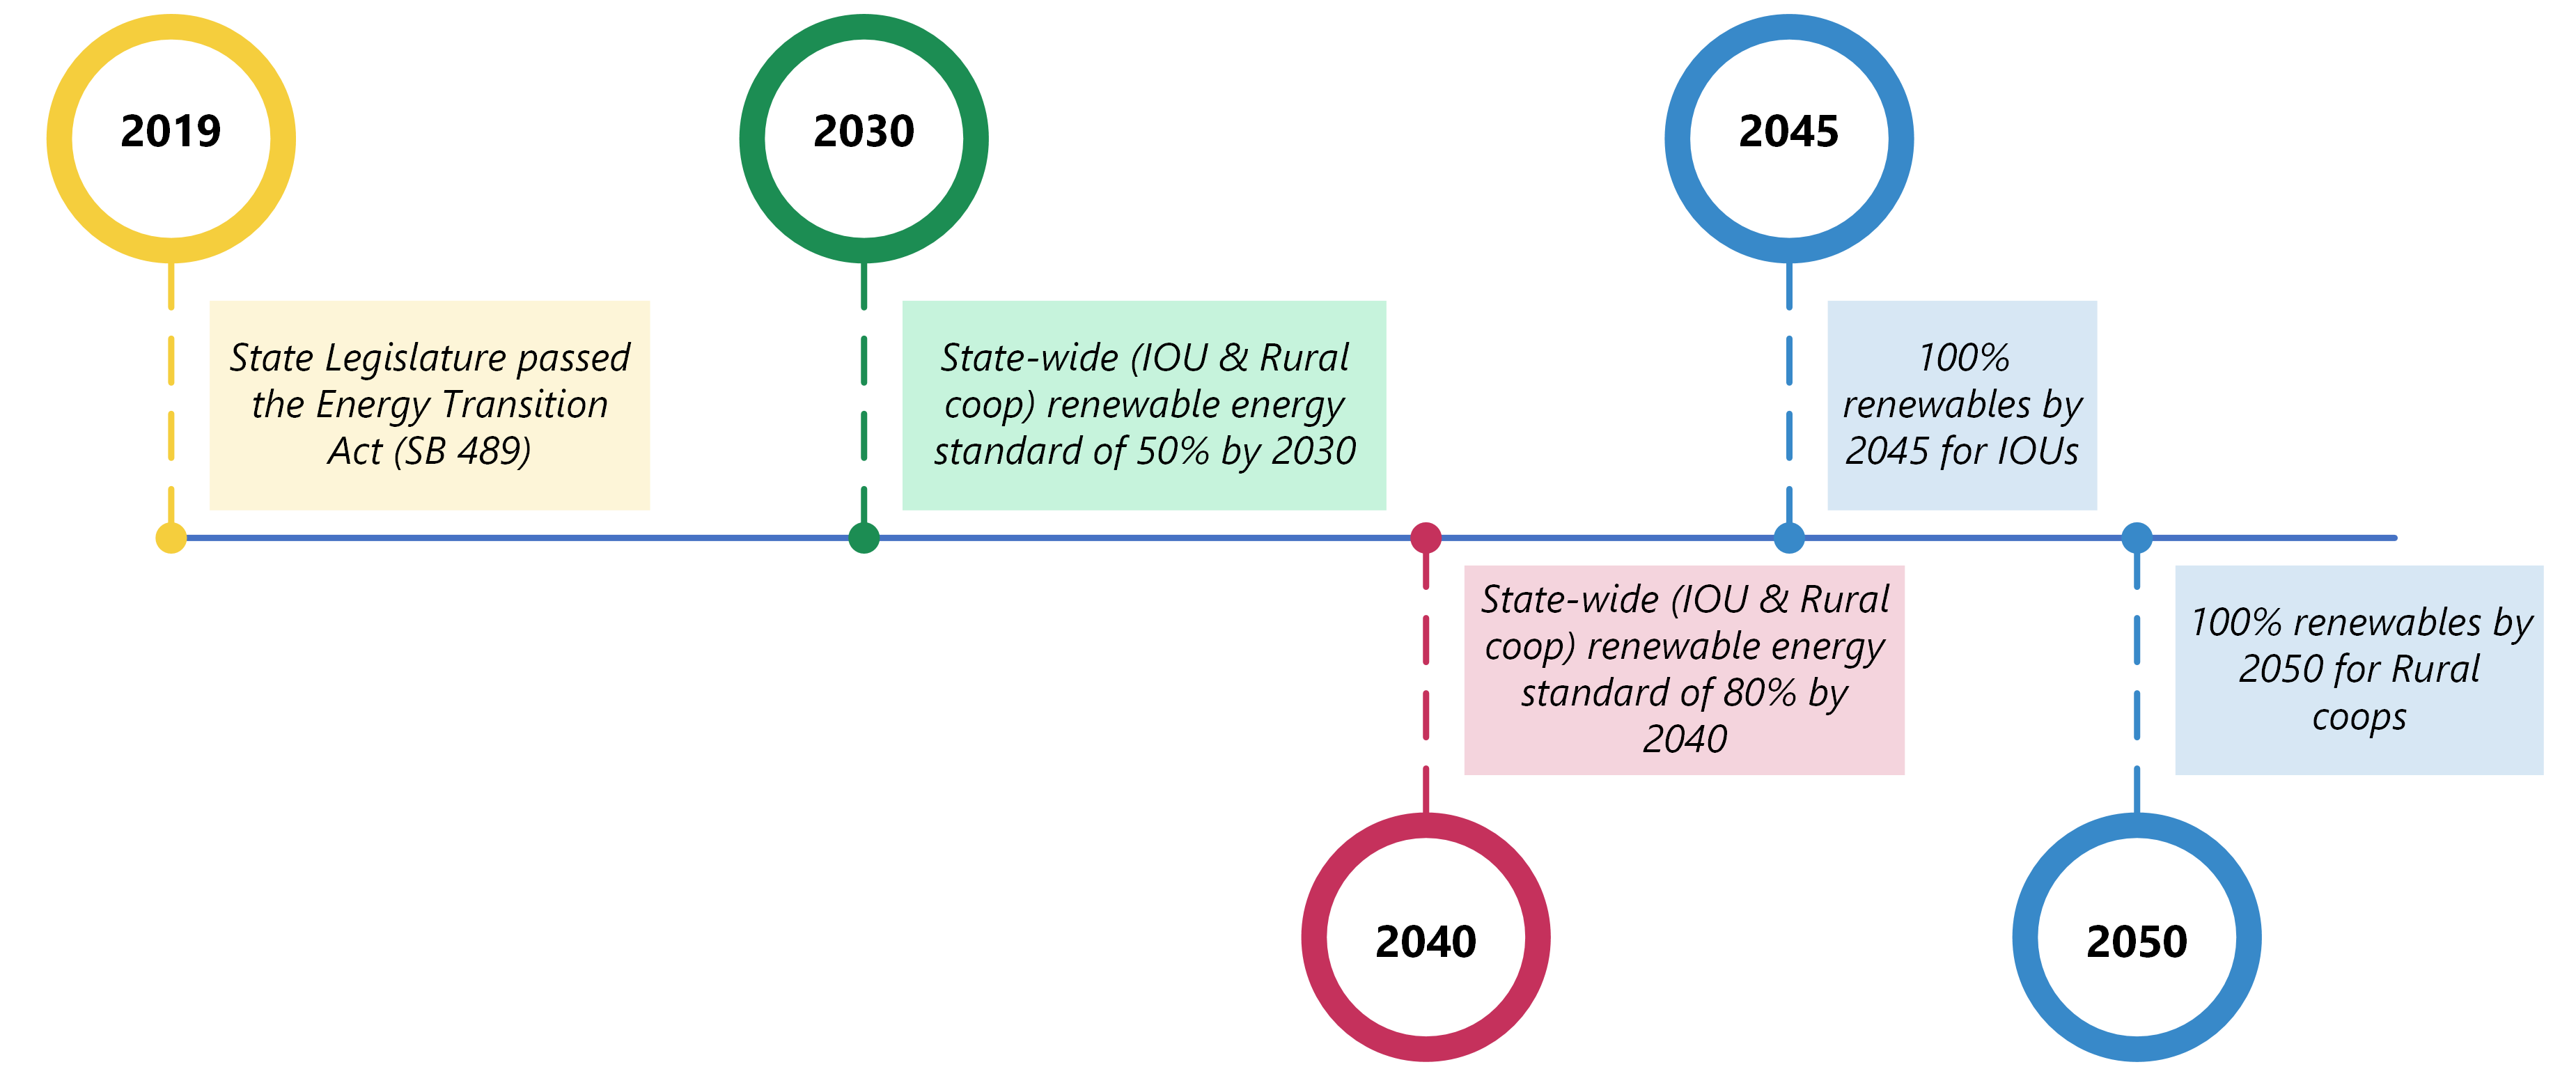
\includegraphics[width=1\textwidth]{figures/nm_eta.png}
    \caption{Timeline of the Energy Transition Act (Senate Bill 489)}
    \label{fig:nm_eta}
\end{figure}

NM is notable for its distinctive demographic composition and climate. Ranking 5th in land area at 121,590 square miles and 36th in population with 2.1 million residents, NM has one of the lowest population density in the nation \parencite{uscensus2022}.\footnote{NM is the 46th most densely populated state in the nation \parencite{uscensus2022}.} NM is also a majority-minority state, with over 50\% of the population identifies as Hispanic and 11.2\% as Native American \parencite{uscensus2020}. [NM Rank XX in GDP per capita in the US; Percentage of population with energy burden higher than 6\%; high variation in income and education.]

NM's economy has been significantly reliant on the oil and gas (O\&G) industry since the discovery of the Permian Basin oil fields in the 1920s. The O\&G industry contributes to around 10\% of NM's annual Gross Domestic Product (GDP) and 25\% and 30\% of the state's tax revenue \parencite{eia2023nm, nmlegislative2023}. This dependency on the fossil fuel industry also poses a challenge in the equitable energy transition.

NM is also well-suited to achieve 100\% renewables as NM boasts abundant wind, solar, and geothermal potential. The state's eastern high plains offer significant wind energy opportunities, while NM ranks third in solar energy potential and sixth in geothermal energy potential nationally. In 2022, renewable sources accounted for 42\% of the state's total electricity generation, well on track to achieve the 2030 50\% renewable target \parencite{eia2023energy}.

The interplay between NM's unique demographics, O\&G dependency, and abundant renewable energy resources underlines the importance of exploring equitable energy transition pathways (Figure \ref{fig:nm_background}) .


\begin{figure}[!ht]
    \centering
    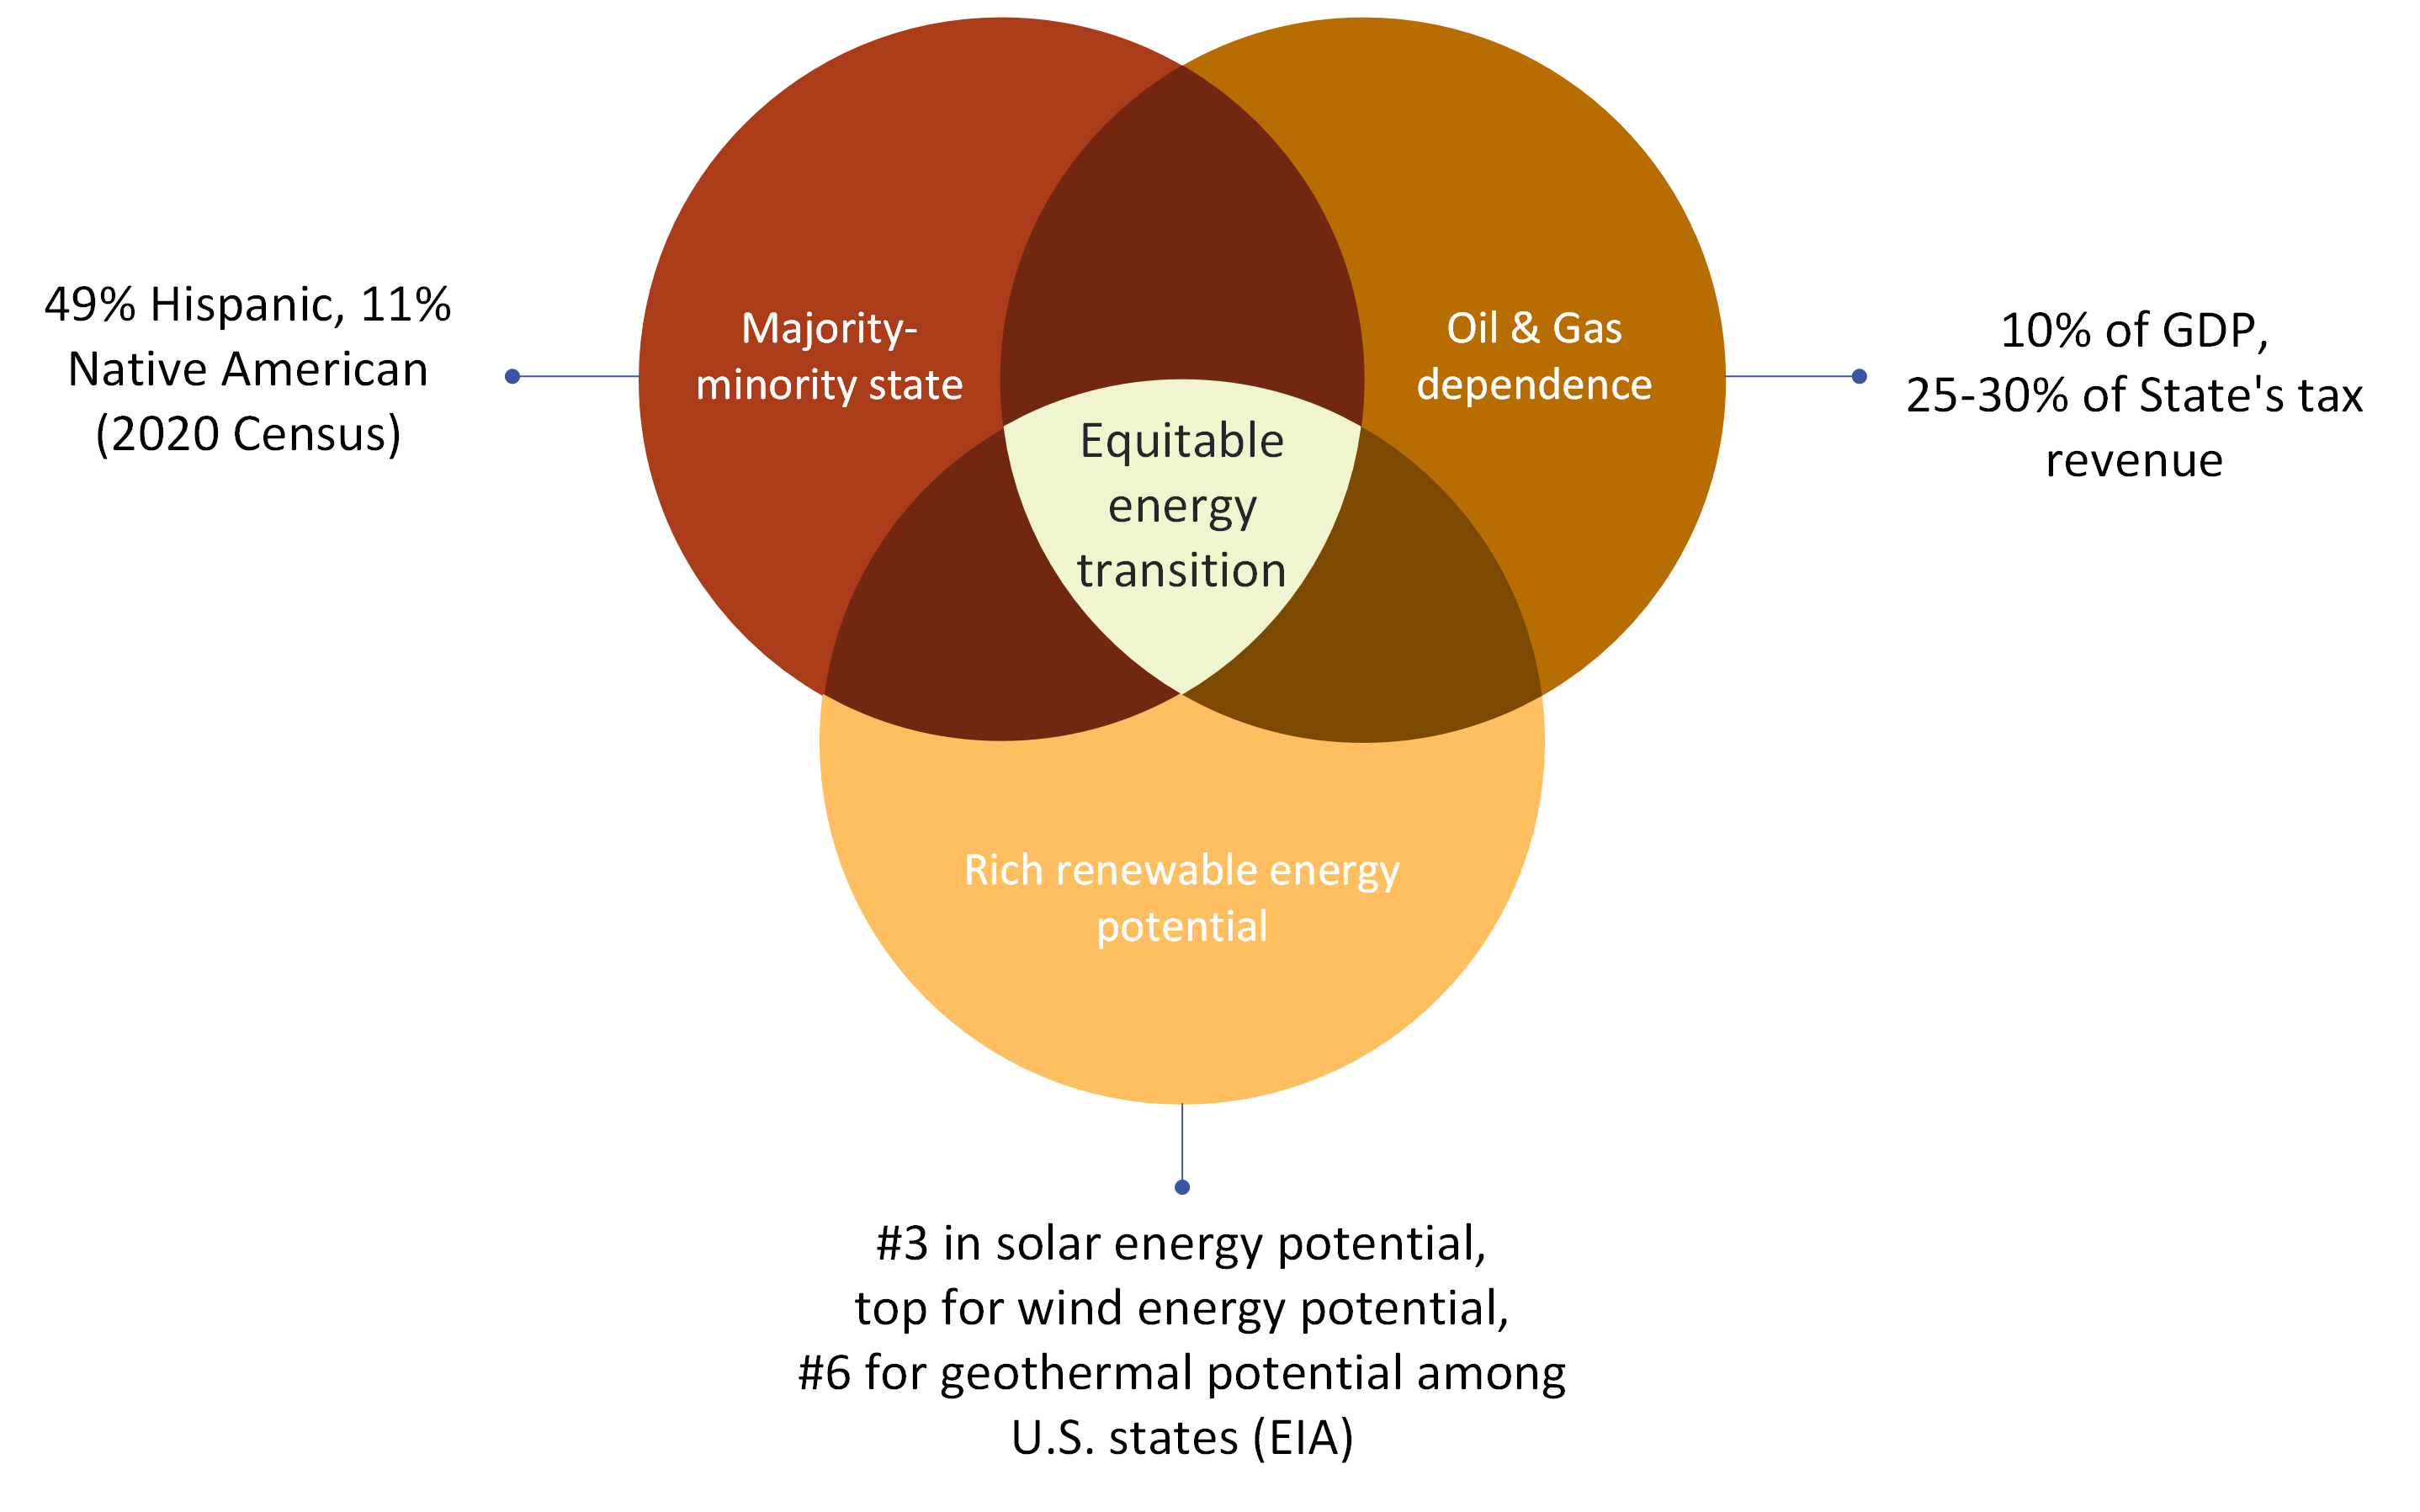
\includegraphics[width=1\textwidth]{figures/nm_background.png}
    \caption{The socioeconomic background of New Mexico}
    \label{fig:nm_background}
\end{figure}

\subsection{Equity in energy transition}

In the context of energy transition, the definition of equity encompasses multiple dimensions. The literature can be categorized into three main aspects of equity, namely \textit{access equity}, \textit{adoption equity}, and \textit{distributional equity}.  

\noindent\textbf{Access equity}

 Access equity refers to the availability and accessibility of solar PV technology for all communities, regardless of income, race, or geographic location. \textcite{brockway2021inequitable} find using California data that existing grid infrastructure may not be sufficiently robust to handle the increased load from widespread solar PV installations without significant upgrades. This can lead to inequitable access, where certain regions or communities might have lesser ability to connect their solar systems to the grid due to these capacity issues. This finding is relevant in the New Mexico context as solar installations are concentrated in urban areas where in some areas grid infrastructure limits solar installations. For example, in parts of Albuquerque and Rio Rancho, the feeder grids are already at maximum capacity.\footnote{See \url{https://pnm.maps.arcgis.com/apps/webappviewer/index.html?id=cbd3bad85fc64f2180dda652e957bacd} for areas with maximum feeder capacity.} Residents in these communities will not be approved for new solar installations until the infrastructure is upgraded.\footnote{In 2021, 2022, and 2023, the Public Service Company of New Mexico (PNM) put 96, 70, and 29 new solar applications on hold, respectively, due to a lack of feeder capacity \parencite{pnm2021,pnm2022,pnm2023}. }
 
 
 This is particularly important for New Mexico, given the state's diverse demographics, including tribal areas. 
 
 
 
 Second is equity in affordability, which evaluates the effectiveness of the state's solar incentives in reducing the financial burden for low- and moderate-income households to adopt solar energy. Without such measures, incentives may only benefit households that would have adopted solar PV regardless of the incentives, due to warm glow or lower long-term energy costs. Third is equity in energy use, which examines how electricity consumption changes with growing solar PV adoption. Research has shown that households that adopt solar PV consume more electricity than before installing solar PV (Deng \& Newton, 2017). This rebound effect in electricity consumption may further increase the cost of electricity for all households and exacerbate energy poverty among low-income households (Cong et al., 2022). 



In the last decade, there is a growth trajectory in solar energy adoption in New Mexico, which shows the increasing awareness and acceptance of solar energy as a viable alternative. 




2. Most existing solar installations are concentrated in metropolitan areas (Albuquerque, Santa Fe, and Las Cruces). This raises the equity question in solar adoption within New Mexico. 



% Could be moved to the motivation part



\subsection[Policy background]{Policy background}

Incentives to promote solar PV adoption in the residential sector have been implemented at different regulatory levels, from federal all the way to the service providing utilities. These incentives play important roles in the decision making of going solar. All incentives are essentially financial, which either lowers the up front cost of solar investment or reduce the payback period of solar. In the remainder of this section, we introduce each incentive, with details on the incentive structure, time of initiation and expiration, eligibility, etc. 

Figure \ref{fig:nm_incentive} summarizes the various incentives offered to solar owners and their respective policy time span.

\begin{figure}[H]
    \centering
    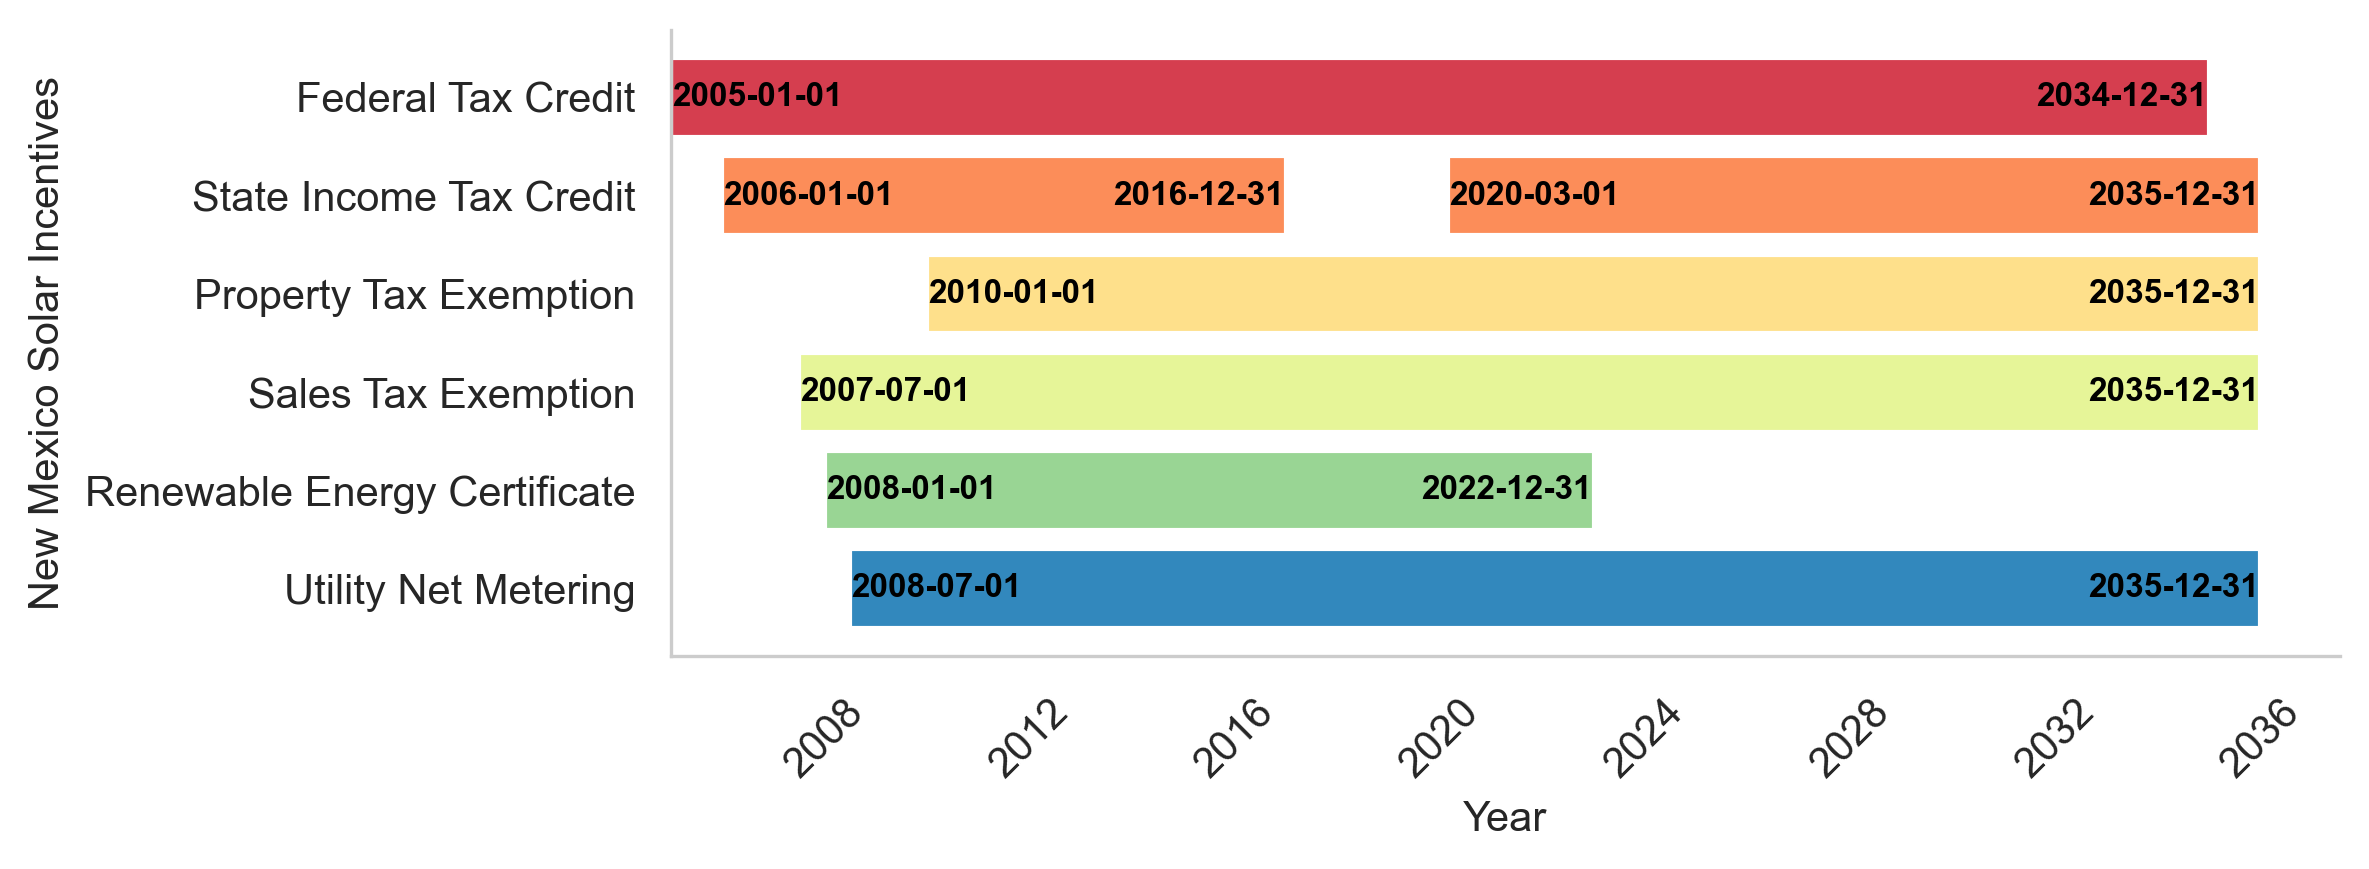
\includegraphics[width=1\textwidth]{figures/policy_timeline.png}
    \caption{Incentives for residential solar PV in New Mexico}
    \label{fig:nm_incentive}
\end{figure}

\subsubsection{Federal incentives}


The federal tax credit for solar panel installations, also known as the Investment Tax Credit (ITC), was initially introduced in the Energy Policy Act of 2005. It provided a tax credit of 30\% for residential and commercial solar energy installations. ITC was extended multiple times and maintained a 30\% credit for solar installations through 2019. The tax credit percentage was stepped down in 2020, where the systems installed in 2020 and 2021 were eligible for a 26\% tax credit \parencite{doeitc}. ITC was originally set to phase down after 2022 (26\% in 2022, 22\% in 2023, 0\% by 2024) before the introduction of the Inflation Reduction Act (IRA) in 2022. IRA extended the ITC, now known as the Residential Clean Energy Credit, which provide a 30\% tax credit from 2022 through 2032. The credit rate phases down to 26\% in 2033 and 22\% in 2034, unless otherwise noted. The federal tax credit place in limit on the total amount claimed, and any credit exceeding tax liability can be carried forward to future tax years \parencite{irs}.

\subsubsection{State incentives}

\textbf{Solar tax credit}

With the growing recognition of the importance of renewable energy as a means to reduce greenhouse gas emissions and combat climate change since the 2000s, NM initiated a solar tax credit in 2006, known as the Solar Market Development Tax Credit (SMDTC). The SMDTC was effective from January 1, 2006, through December 31, 2016, and offered 10\% tax credit on the total installation costs of solar panel systems, with a maximum credit amount of \$9,000 per taxpayer per taxable year. The SMDTC was reinstated in 2020, known as the New Solar Market Development Tax Credit (NSMDTC). Solar PV systems installed after March 1st, 2020 are eligible for a 10\% tax credit on the total installation costs with a maximum credit amount of \$6,000. The total tax credit issued within the state is capped at 8 million dollars for the tax years 2020  and 2021, and 12 million dollars after 2022.\footnote{In both 2021 and 2022, the credit cap was reached. \url{https://nm-emnrd.maps.arcgis.com/apps/dashboards/e882d2ccd57e4a99bc6d2a4314fcd3bb}} There is no income threshold to claim the tax and all credit exceeding the taxpayers' liability are refunded instead of carrying over to subsequent tax years \parencite{nmsmdtc}. 

\noindent\textbf{Property tax exemption}

Under House Bill 233 of the NM legislature, enacted in 2010, residential solar systems will not be treated as physical improvements and therefore will not increase the value of the property for property tax purposes. Future assessments, however, can include the value of a solar energy system if the property is sold \parencite{propertytax}. This exemption provides an financial incentive for homeowners since the installation of solar PV will increase the value of the property on the housing market without having to pay the additional property tax.


\noindent\textbf{Sales tax exemption}

The NM Gross Receipts Tax Exemption policy for solar energy systems, effective in 2007, allows businesses to deduct receipts from selling solar equipment or installation services
\parencite{NMStat2021}. Essentially, for consumers, there is no sales tax on top of the cost of solar installation which reduces the financial burden of solar adopters.


\noindent\textbf{Renewable energy certificates}

The New Mexico Renewable Energy Certificate (REC) policy for solar PV is part of the state's broader Renewable Portfolio Standard (RPS). The RPS mandates that IOUs must secure 50\% of their capacity through carbon-free renewables by 2030 and 100\% by 2045. For rural electric cooperatives, the goals are 40\% by 2025, 50\% by 2030, and 100\% by 2050. The IOUs in NM thus offered Renewable Energy Certificate (REC) purchase agreements to solar owners for a limited time to count residential solar generation towards their required RPS. The Public Service Company of New Mexico (PNM) offered a Solar Renewable Energy Certificate (SREC) program that awards systems a stepped purchased rate for the energy generated for residential systems. This program was discontinued by the end of 2022 \parencite{pnmrec}. The El Paso Electric Company (EPE) offered a tiered REC purchase rate for systems install before 2017, which ended on December 31, 2020 \parencite{eperec, eperecmid}.\footnote{Details on the purchase agreements can be found on the respective company's websites.}

\subsubsection{Utility incentives}

Utility companies (IOUs, rural cooperatives, and public utilities) in NM are mandated by the NM Public Regulatory Commission (NM PRC) to offer net metering programs to solar customers. Under net metering, solar customers who generate excess electricity with their solar panel systems can send it back to the grid and receive credits. These credits can be used to offset future electricity usage.\footnote{For example, if the solar panels are generating during the day and the household is consuming less than production, the electricity will be sold back to the grid for a credit, i.e., the meter will turn backwards. At night, solar is not producing and the household consumes grid electricity, i.e., the meter run forward.} However, the details of the net metering program vary by utility. For example, PNM offers a net metering program for all residential solar systems for their billing cycle. For small PV systems (inverter capacity lower than 10kW-AC), Any excess generation for the month (monthly usage is lower than total monthly generation) is credited to the customer's account and can be used for future billing cycles and never expires, unless the account is closed. The excess generation from large PV systems (inverter capacity above than 10kW-AC) is paid each month at the predetermined energy purchase rate for a given month \parencite{pnmnet}. EPE offers net metering for all systems within a billing cycle but all excess generation for the month will be paid out to the customers at the predetermined purchase rate \parencite{epenet,epenetmid}.  The purchase rate of the credits are typically lower than the retail electricity price for all utilities.\footnote{For example, the PNM power purchase rate is 3 to 12 cents per kWh depending on the month of the year in 2023. The retail rate is 7.8 cents per kWh for the first 450 kWh per month and goes up to 15 cents per kWh.}


\newpage
%%%%%%%%%%%%%%%%%%%%%%%%%%%%%%%%%%%%
\section[Current trend]{Current trend of solar PV adoption in New Mexico}

Total installation count

\begin{figure}[H]
    \centering
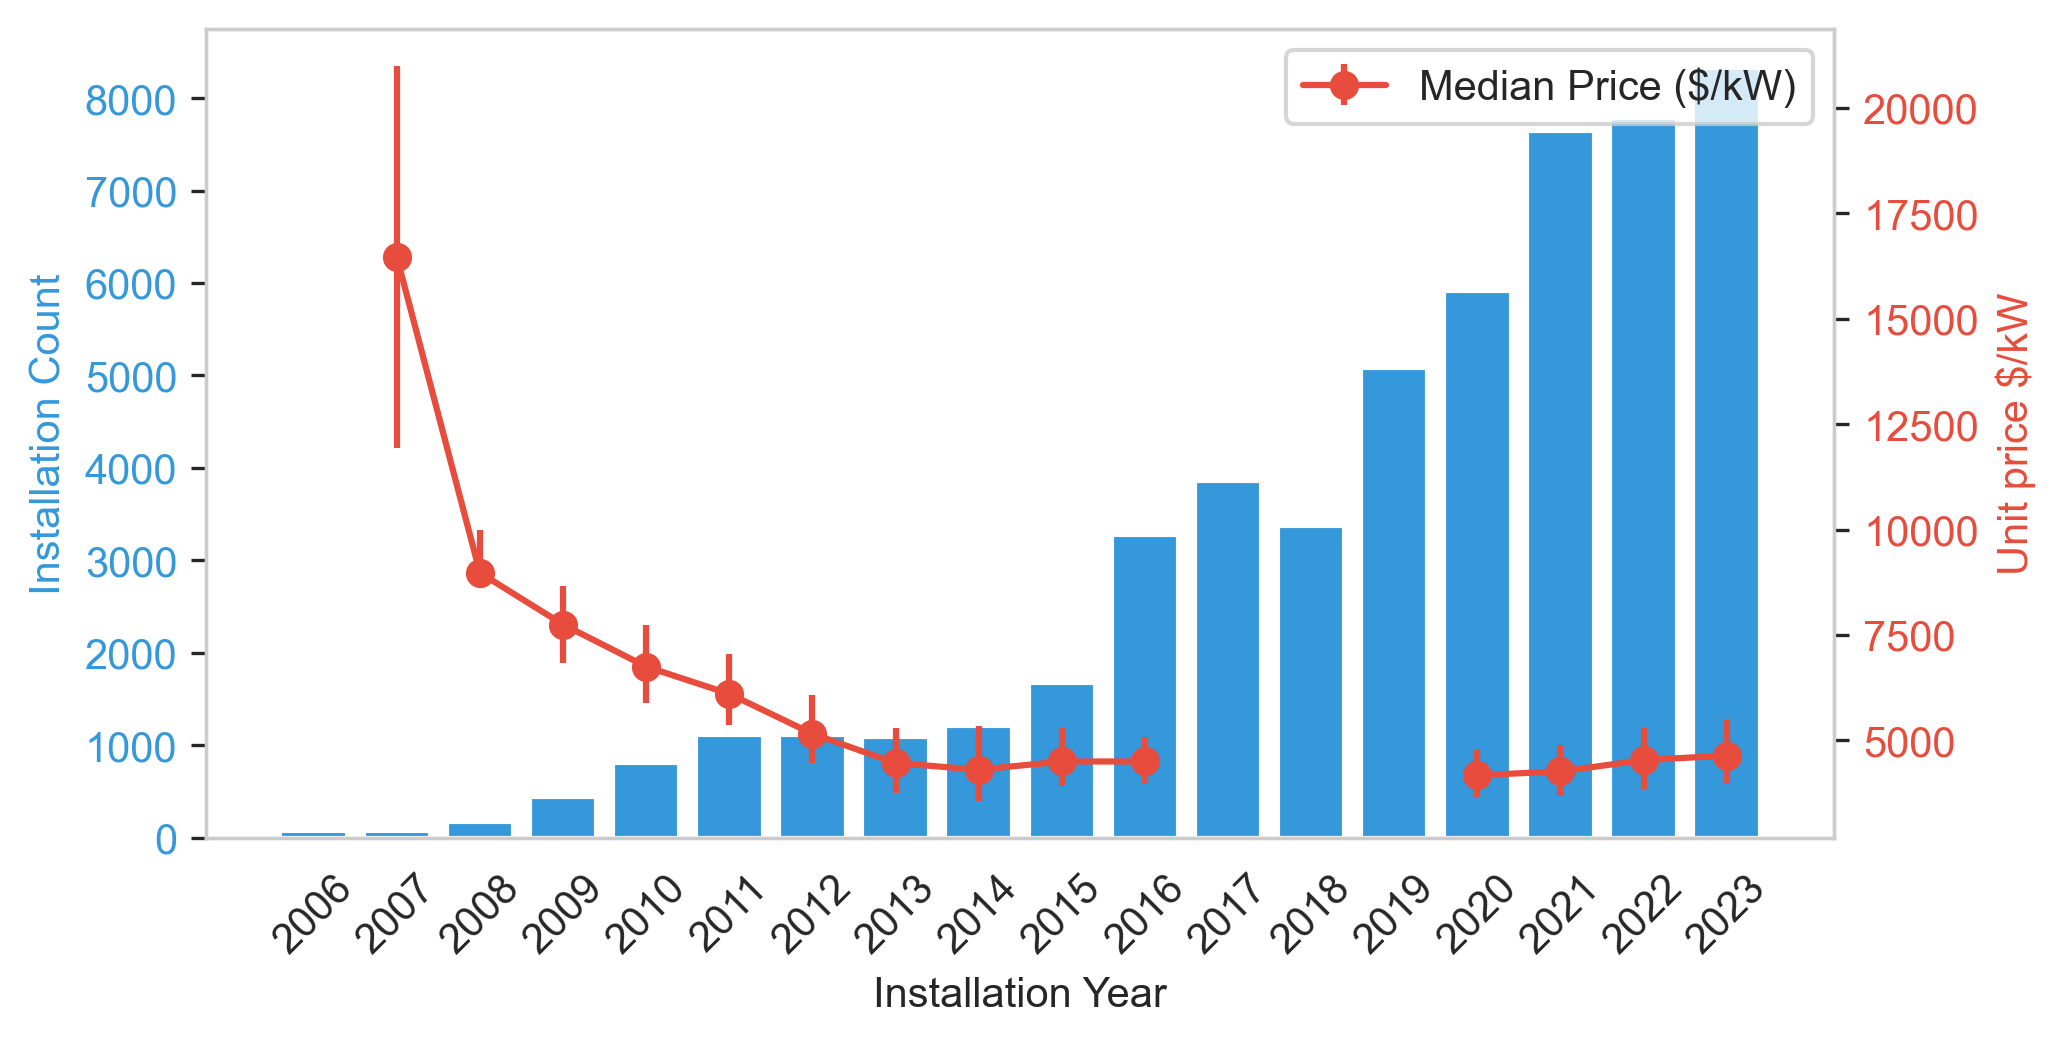
\includegraphics[width=1\textwidth]{figures/installation_count_price.png}
    \caption{Annual solar installation count and unit price in New Mexico}
    \label{fig:installation_count}
    \begin{flushleft}
        \footnotesize Note: The whiskers show 25\% to 75\% range of the unit prices. The installed price ranges exclude any systems with battery storage.
    \end{flushleft}
    
\end{figure}

\begin{figure}[!ht]
    \centering
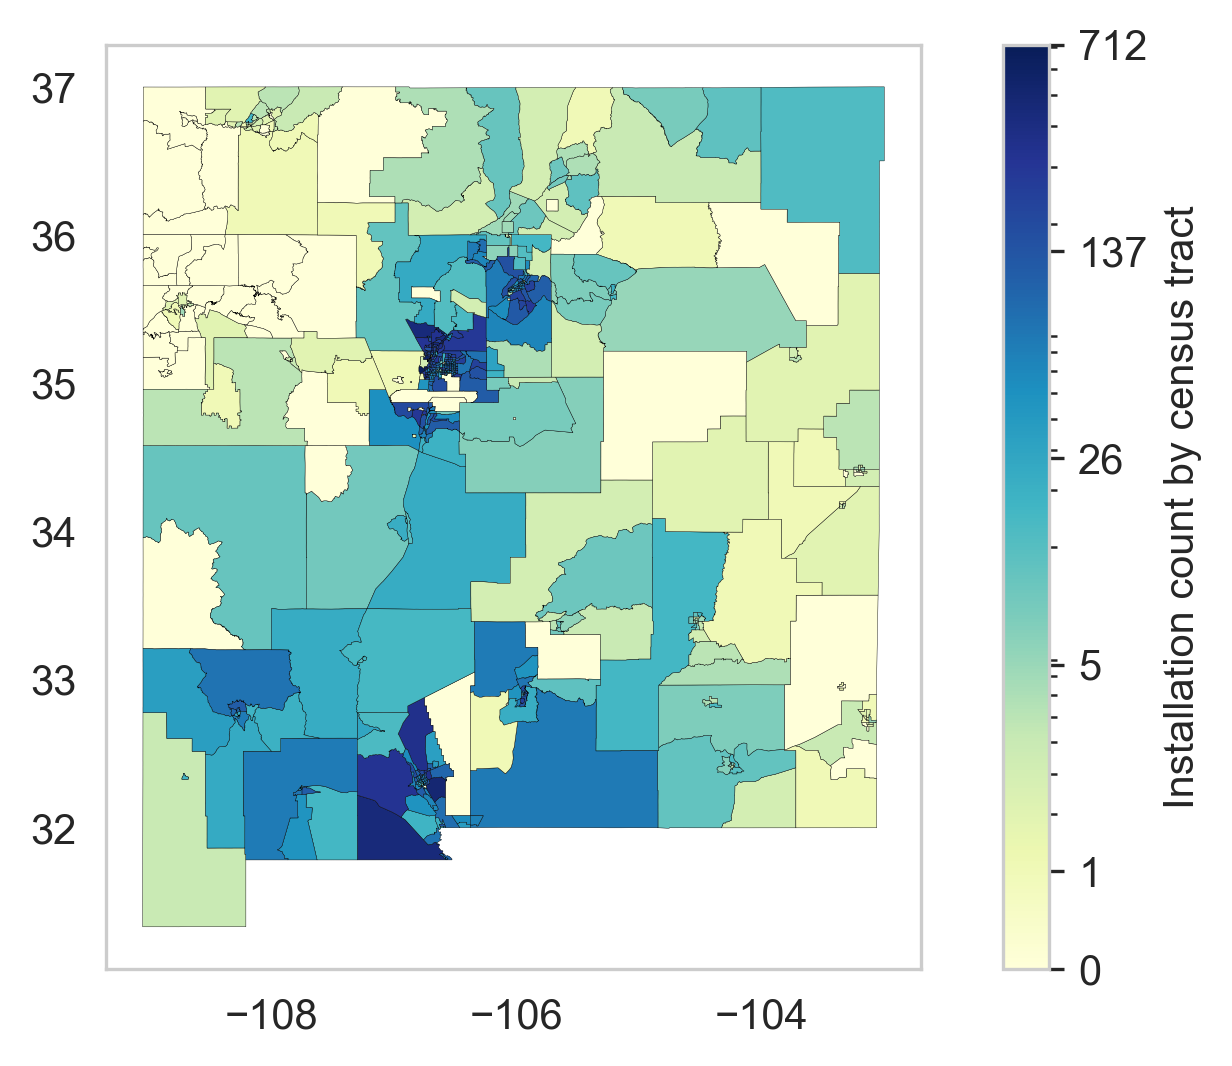
\includegraphics[width=0.7\textwidth]{figures/tract_count_map.png}
    \caption{Total installation count by 2020 census tract}
    \label{fig:tract_map}
    
\end{figure}

\begin{figure}[!ht]
    \centering
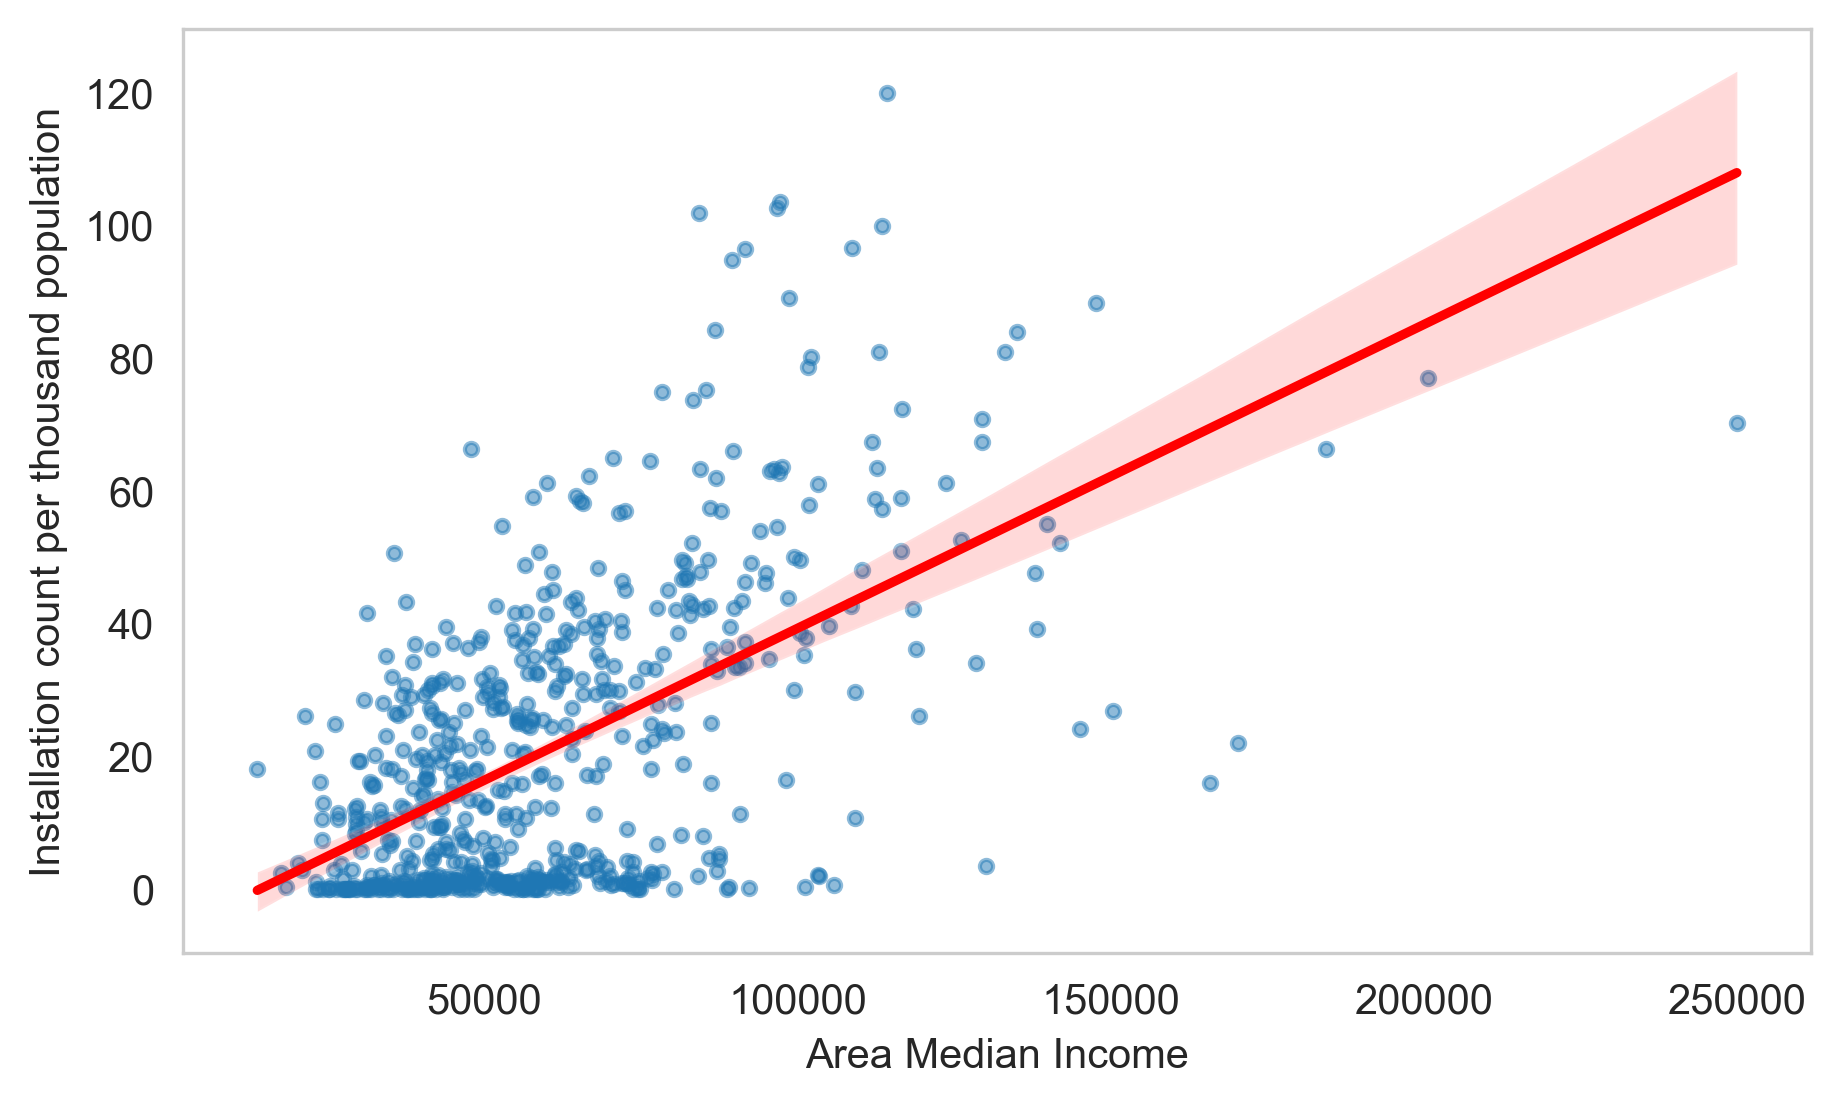
\includegraphics[width=1\textwidth]{figures/population_ami_count.png}
    \caption{Installation per thousand population by area median income}
    \label{fig:tract_map}
        \begin{flushleft}
        \footnotesize Note: The population and area median income (AMI) are taken at the 2022 level.
    \end{flushleft}
\end{figure}

\begin{figure}[!ht]
    \centering
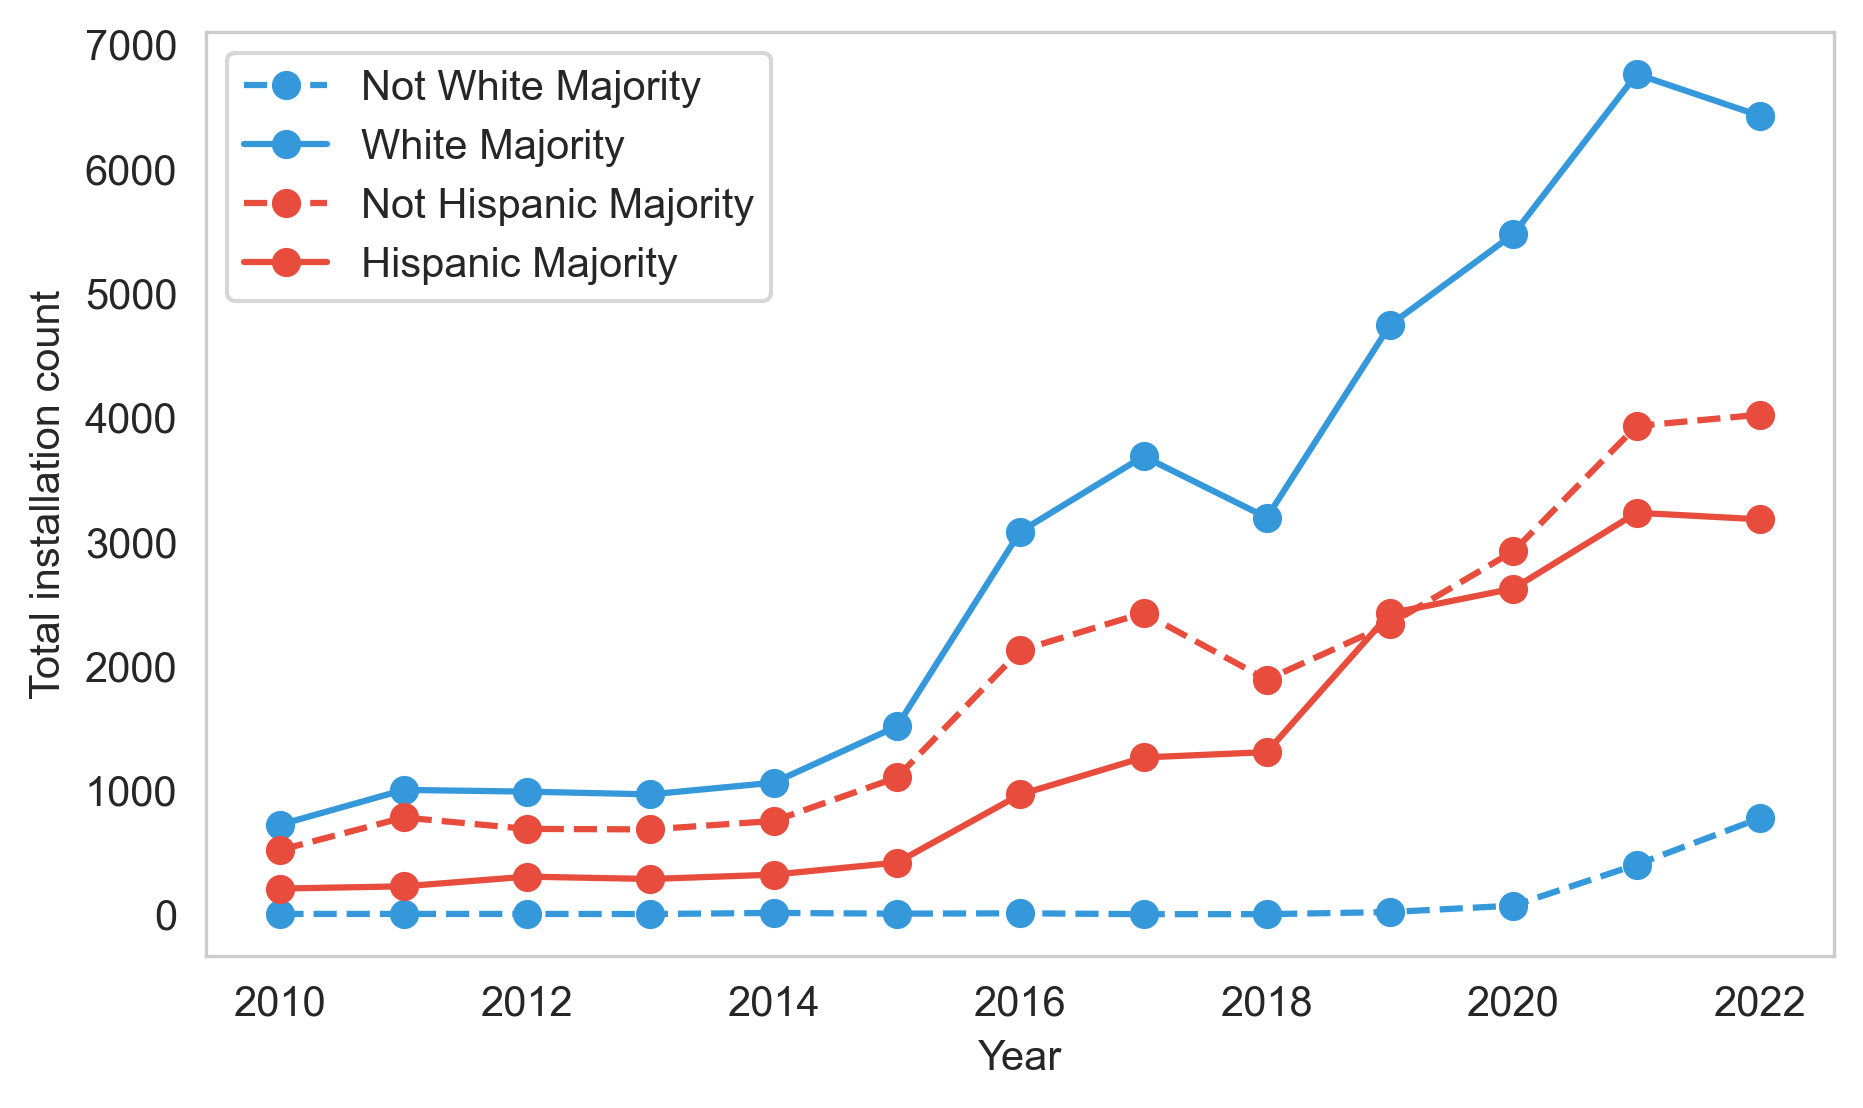
\includegraphics[width=1\textwidth]{figures/installation_by_race.png}
    \caption{Annual installation by racial majority group}
    \label{fig:installation_race}
        \begin{flushleft}
        \footnotesize Note: White majority refers to census tracts with more than 50\% population identified as white. Hispanic majority refers to census tracts with more than 50\% population identified as Hispanic. 
    \end{flushleft}
\end{figure}

\begin{figure}[!ht]
    \centering
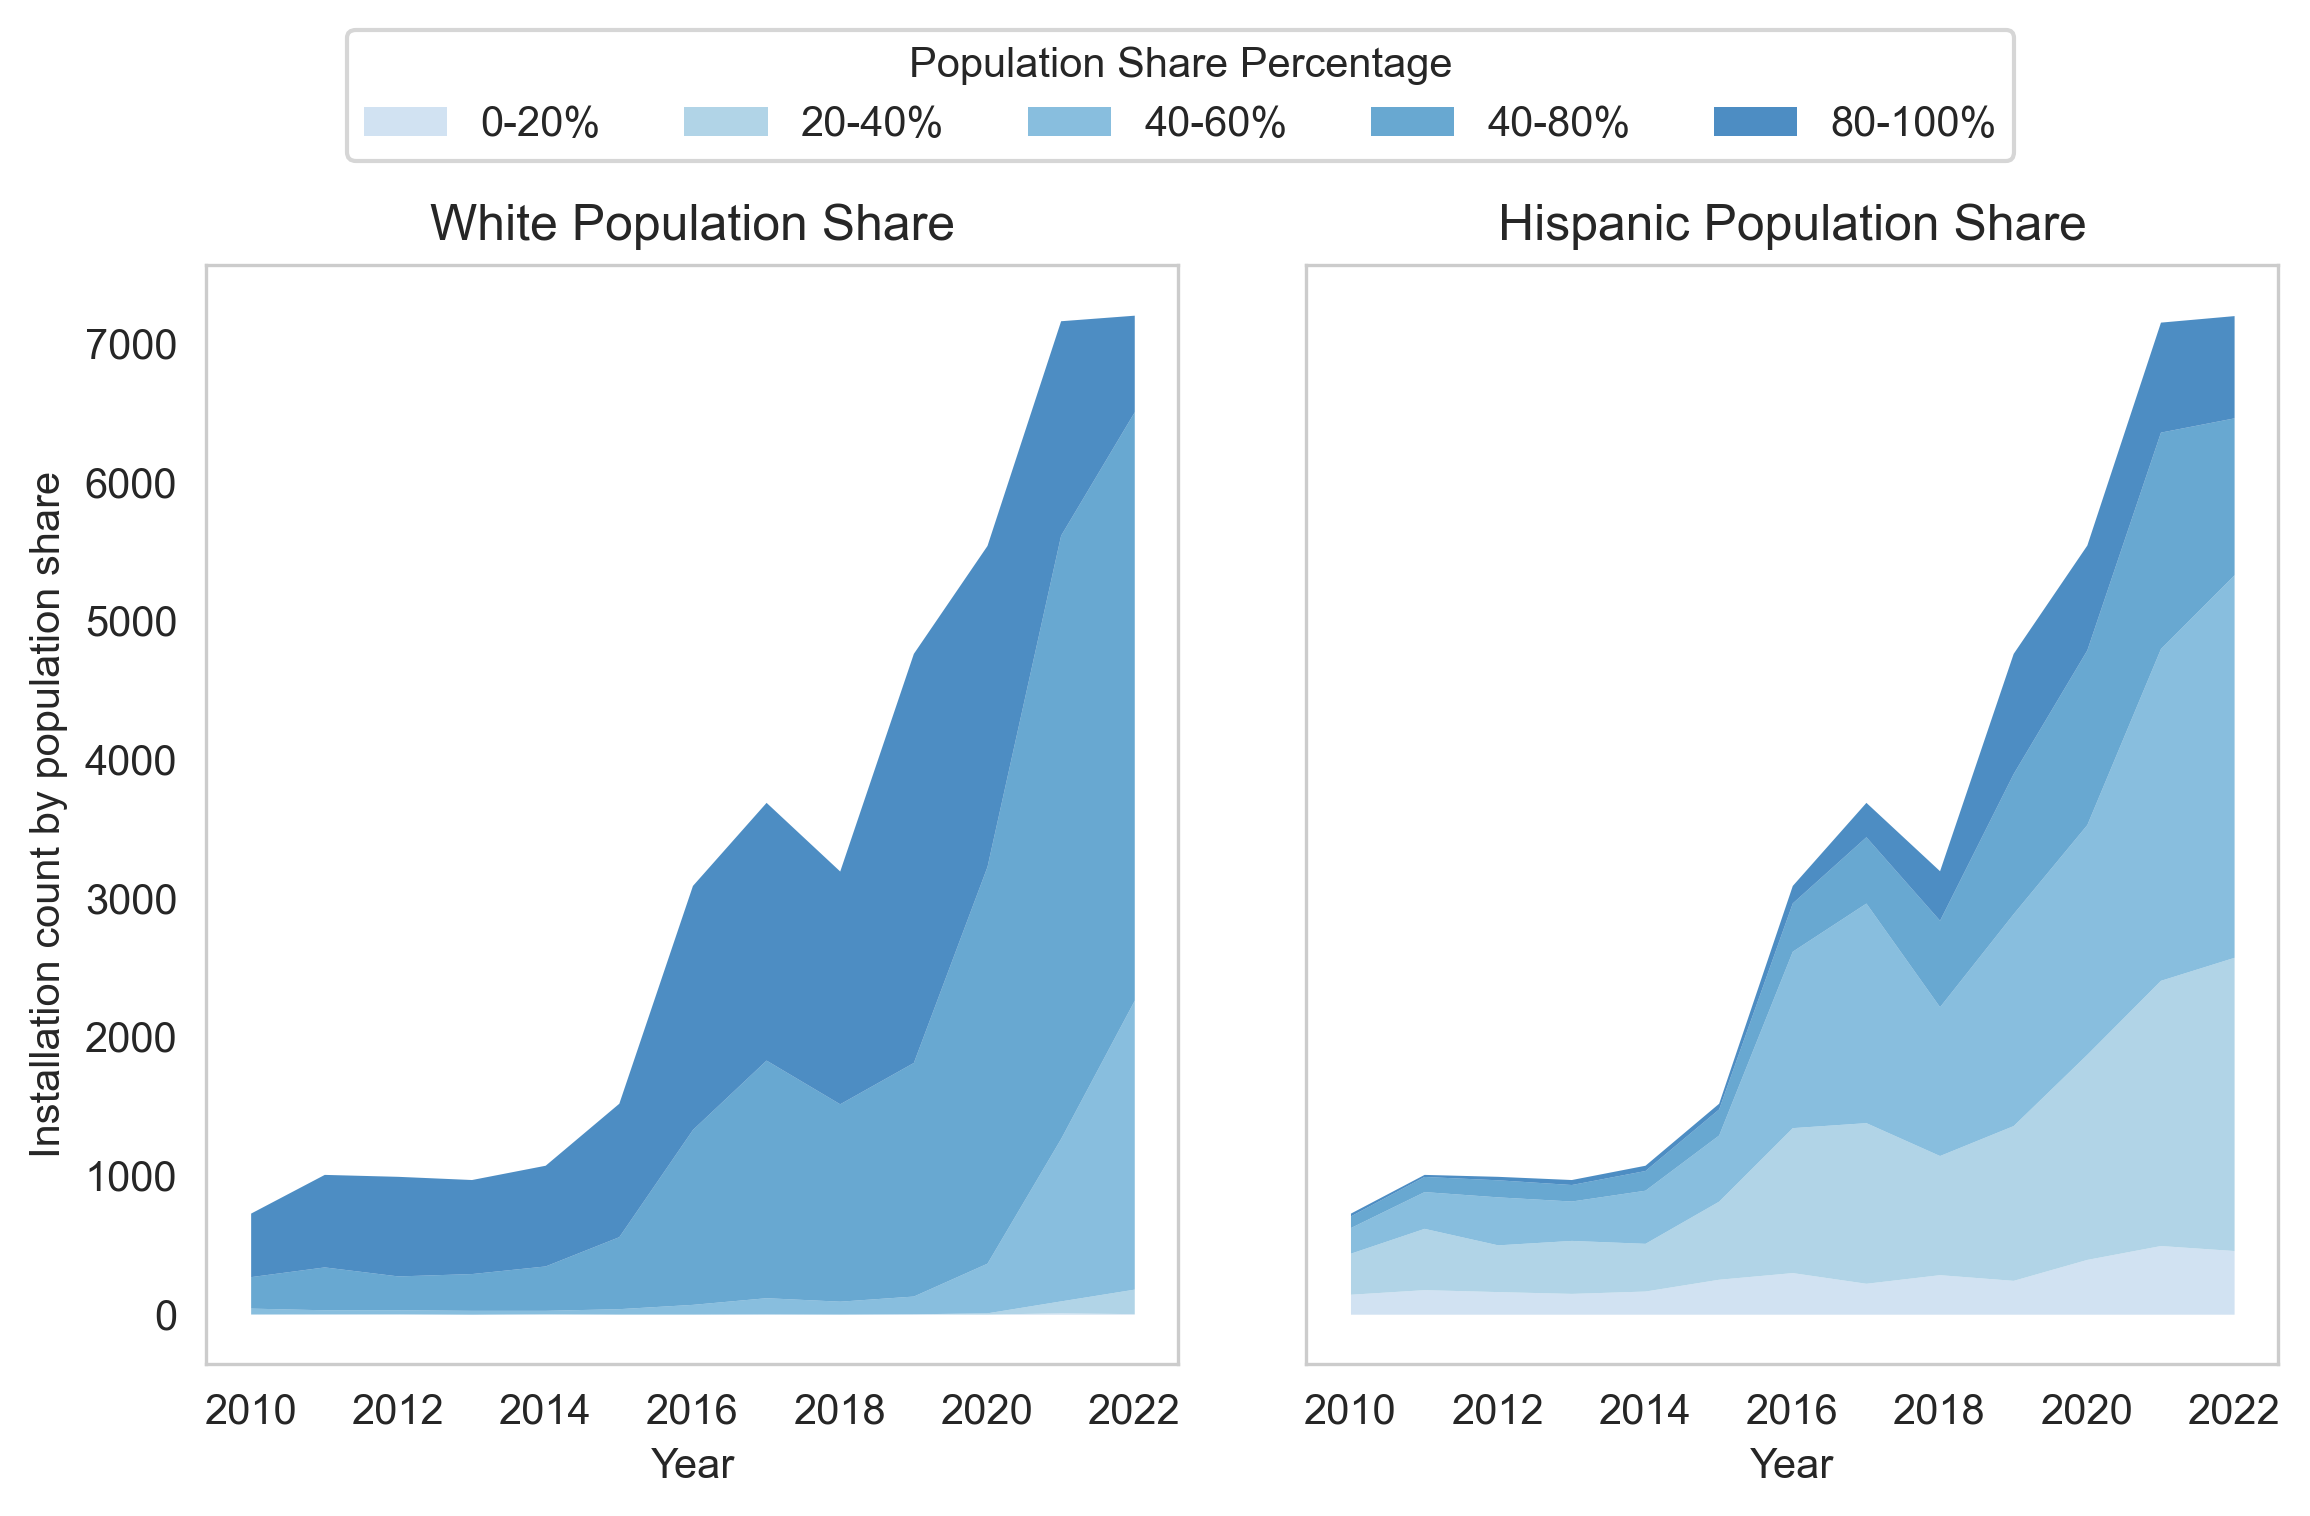
\includegraphics[width=1\textwidth]{figures/population_quintiles.png}
    \caption{Installation by racial population share}
    \label{fig:population_quintiles}
    %     \begin{flushleft}
    %     \footnotesize Note: White majority refers to census tracts with more than 50\% population identified as white. Hispanic majority refers to census tracts with more than 50\% population identified as Hispanic. 
    % \end{flushleft}
\end{figure}

\begin{figure}[!ht]
    \centering
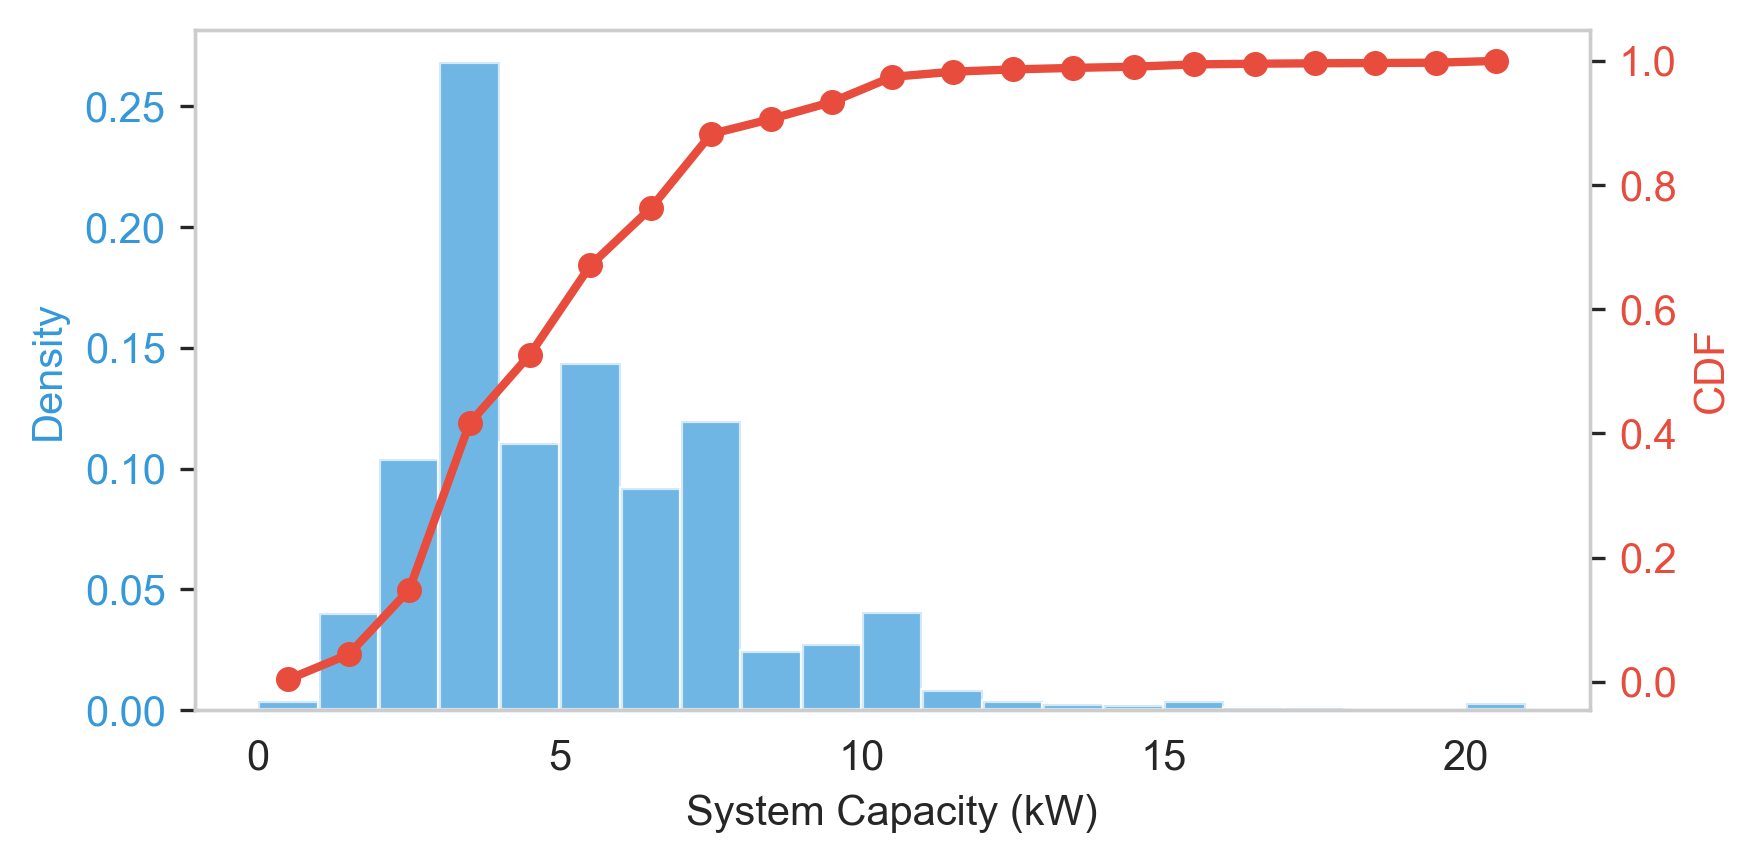
\includegraphics[width=1\textwidth]{figures/capacity_density_cdf.png}
    \caption{Distribution  of installed solar PV system capacity}
    \label{fig:capacity_density}
        \begin{flushleft}
        \footnotesize Note: Systems with capacity greater or equal to 20kW are grouped together. 
    \end{flushleft}
\end{figure}

\begin{figure}[!ht]
    \centering
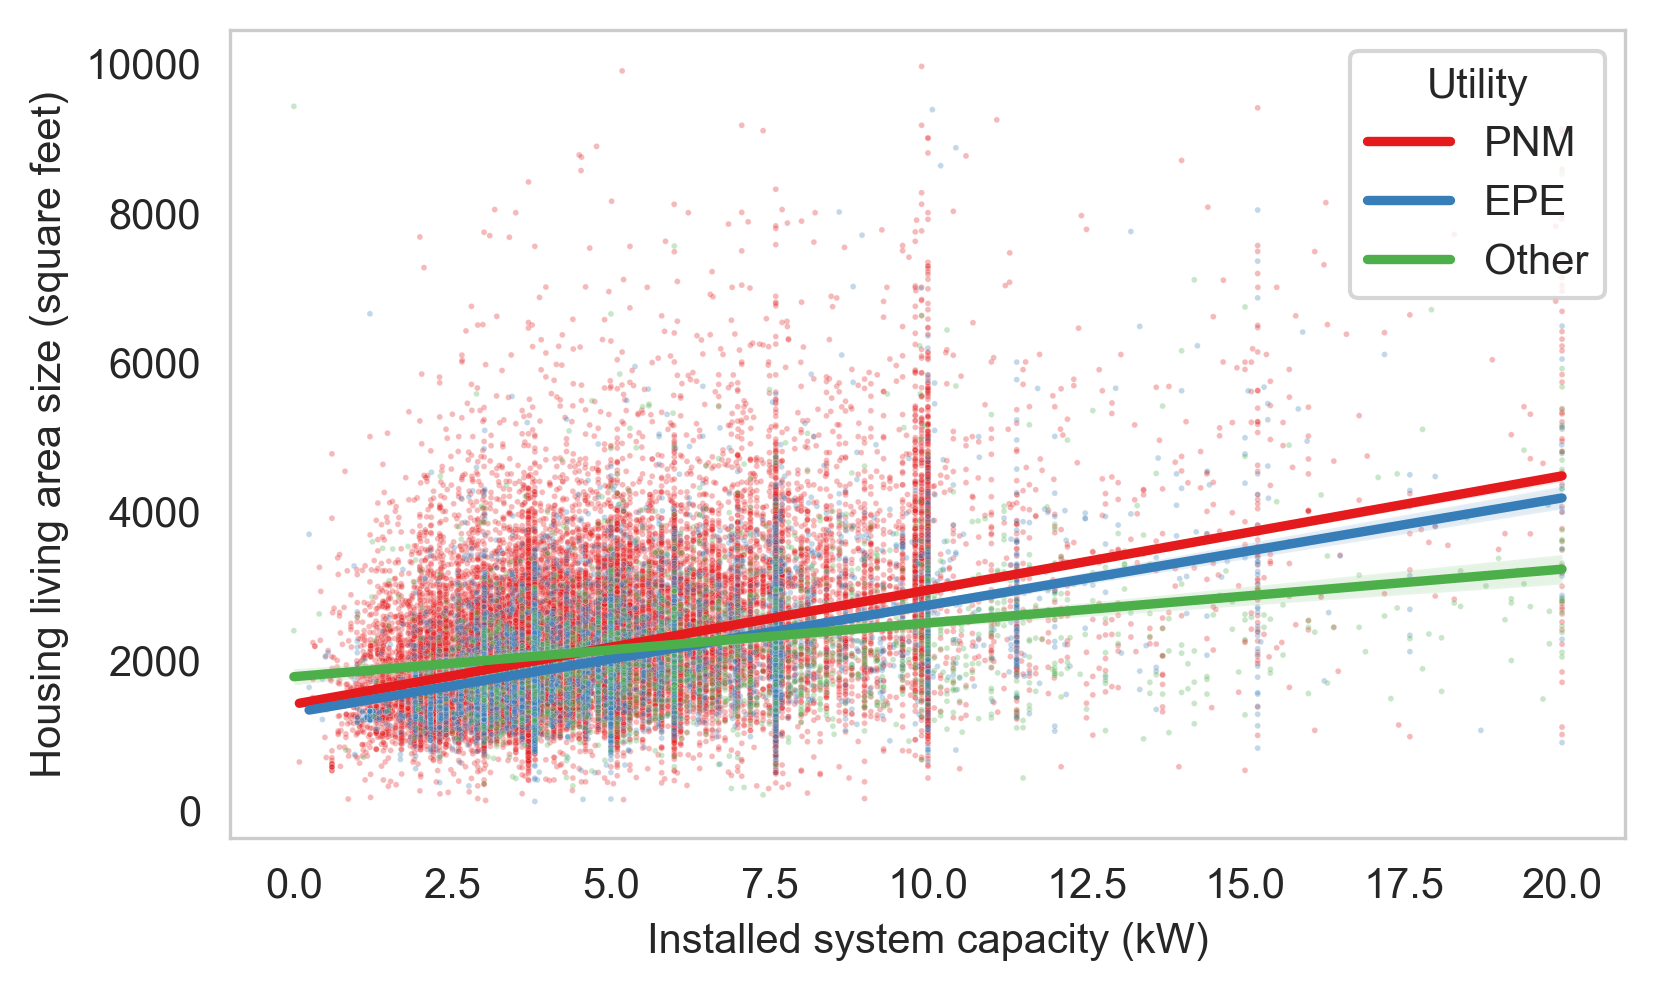
\includegraphics[width=1\textwidth]{figures/capacity_house_size.png}
    \caption{Linear relationship between installed capacity and housing size}
    \label{fig:capacity_size}
    %     \begin{flushleft}
    %     \footnotesize Note: Systems with capacity greater or equal to 20kW are grouped together. 
    % \end{flushleft}
\end{figure}


\begin{figure}[!ht]
    \centering
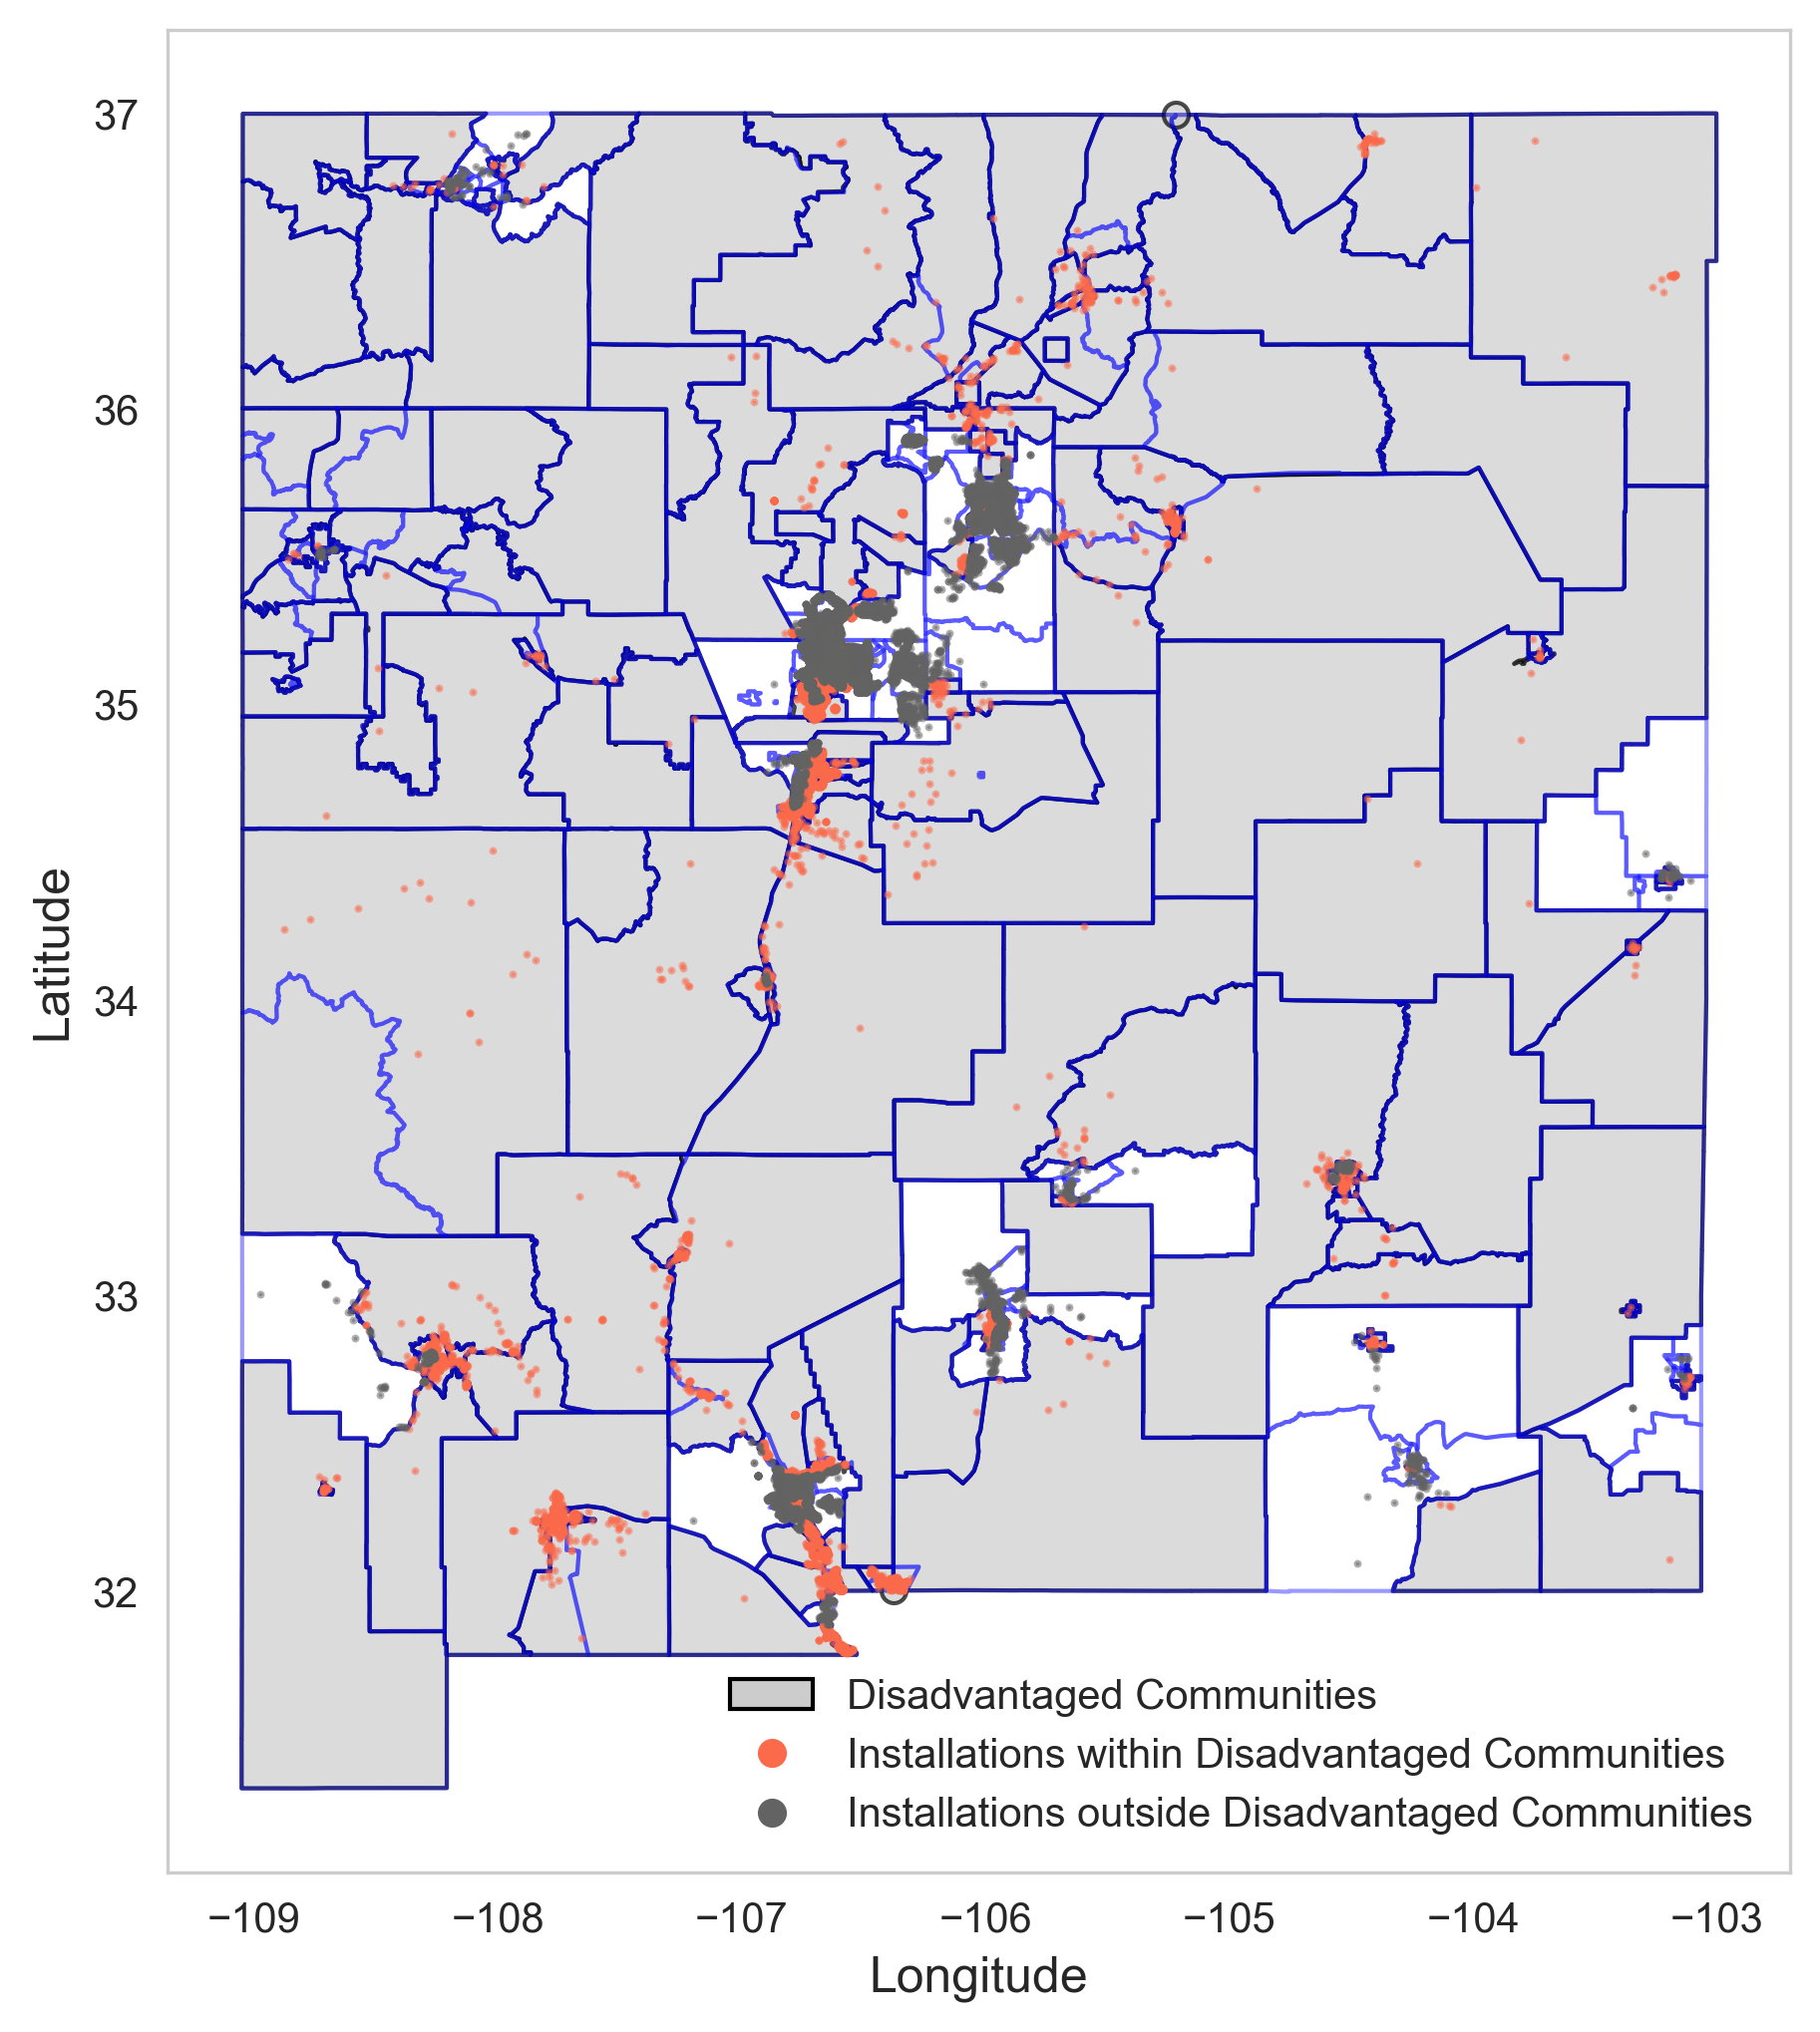
\includegraphics[width=0.7\textwidth]{figures/disadvantage_installation.png}
    \caption{Installation within and outside disadvantaged communities}
    \label{fig:disadvantage_installation}
        \begin{flushleft}
        \footnotesize Note: Disadvantage communities shape file retrieved from the Climate and Economic Justice Screening Tool \url{https://screeningtool.geoplatform.gov/en/#10.84/36.2534/-104.868}. Census tracts that are overburdened and underserved are highlighted as being disadvantaged on the map.
    \end{flushleft}
\end{figure}


\newpage
%%%%%%%%%%%%%%%%%%%%%%%%%%%%%%%%%%%
\section[Adoption equity]{Adoption equity of solar PV}
% Section on the tract-level analysis

\subsection{Data}


\subsection{Methodology}
\subsection{Results}


\newpage
%%%%%%%%%%%%%%%%%%%%%%%%%%%%%%%%%%%
\section[Distribution equity]{Distribution equity of solar PV}
% Section on credit claim

\subsection{Data}
\subsection{Methodology}



\subsection{Results}

\begin{table}[!ht]
    \centering
    \resizebox{1\textwidth}{!}{
   \begin{tabular}{lrrrrr}
\hline
                                         &   count &      mean &       std &   min &      max \\
\hline
 State credit                            &   26735 &      0.44 &      0.50 &     0 &        1 \\
 System capacity                         &   26735 &      5.09 &      2.51 &     0 &       43 \\
 \# of Bedrooms                           &   25951 &      3.33 &      0.78 &     0 &       17 \\
 Zestimate                               &   26087 & 483442.77 & 348557.87 & 49600 & 14324300 \\
 Housing size (sq ft)                    &   26735 &   2201.28 &    975.74 &   100 &    24517 \\
 Year built                              &   26397 &   1989.18 &     21.99 &  1750 &     2024 \\
 \% population with bachelor degree (\ensuremath{>}25) &   26735 &      0.37 &      0.17 &     0 &        0 \\
 Owner occupancy rate                    &   26735 &      0.61 &      0.23 &     0 &        1 \\
 Mortgage rate                           &   26735 &      0.41 &      0.17 &     0 &        0 \\
 Area Median Income                      &   26735 &  69062.99 &  27312.01 & 12014 &   250000 \\
 Population                              &   26735 &   4904.32 &   2235.43 &   274 &    15722 \\
 Median Age                              &   26735 &     41.07 &      8.80 &    20 &       82 \\
 \% population identified as White        &   26735 &      0.83 &      0.09 &     0 &        1 \\
 \% population identified as Hispanic     &   26735 &      0.47 &      0.21 &     0 &        1 \\
 Urban share                             &   26735 &      0.86 &      0.28 &     0 &        1 \\
\hline
\end{tabular}}
    \caption{Summary statistics}
    \label{tab:sumstat}
\end{table}

\begin{table}[!htbp] \centering
  \caption{Regression results of linear probability model for state credit claim}
  \resizebox{1\textwidth}{!}{
\begin{tabular}{@{\extracolsep{5pt}}lccccc}
\\[-1.8ex]\hline
\hline \\[-1.8ex]
& \multicolumn{5}{c}{\textit{Dependent variable: State Credit}} \
\cr \cline{2-6}
\\[-1.8ex] & (1) & (2) & (3) & (4) & (5) \\
\hline \\[-1.8ex]
 System capacity & -0.006$^{***}$ & 0.003$^{*}$ & 0.010$^{***}$ & 0.009$^{***}$ & 0.008$^{***}$ \\
& (0.001) & (0.001) & (0.001) & (0.001) & (0.001) \\
 Log Zestimate & 0.301$^{***}$ & 0.150$^{***}$ & 0.119$^{***}$ & 0.135$^{***}$ & 0.152$^{***}$ \\
& (0.009) & (0.012) & (0.011) & (0.012) & (0.015) \\
 Year built & -0.002$^{***}$ & -0.000$^{}$ & -0.001$^{***}$ & -0.001$^{***}$ & -0.001$^{***}$ \\
& (0.000) & (0.000) & (0.000) & (0.000) & (0.000) \\
 Log Housing size (sq ft) & 0.004$^{}$ & 0.029$^{*}$ & 0.004$^{}$ & -0.005$^{}$ & -0.013$^{}$ \\
& (0.012) & (0.014) & (0.013) & (0.013) & (0.015) \\
 \# of Bedrooms & & -0.017$^{***}$ & -0.009$^{*}$ & -0.009$^{*}$ & -0.010$^{*}$ \\
& & (0.005) & (0.004) & (0.004) & (0.004) \\
 \% population with bachelor degree (>25) & & 0.188$^{***}$ & 0.265$^{***}$ & 0.217$^{***}$ & 0.189$^{***}$ \\
& & (0.033) & (0.031) & (0.034) & (0.037) \\
 Owner occupancy rate & & -0.388$^{***}$ & 0.140$^{***}$ & 0.135$^{***}$ & 0.137$^{***}$ \\
& & (0.021) & (0.025) & (0.025) & (0.025) \\
 Mortgage rate & & -0.289$^{***}$ & -0.280$^{***}$ & -0.267$^{***}$ & -0.223$^{***}$ \\
& & (0.031) & (0.030) & (0.031) & (0.031) \\
 Log Area Median Income & & 0.081$^{***}$ & -0.002$^{}$ & 0.008$^{}$ & 0.010$^{}$ \\
& & (0.013) & (0.014) & (0.014) & (0.014) \\
 Log Population & & 0.056$^{***}$ & 0.017$^{*}$ & 0.016$^{*}$ & 0.025$^{***}$ \\
& & (0.007) & (0.007) & (0.007) & (0.007) \\
 Log Median Age & & 0.046$^{*}$ & 0.007$^{}$ & 0.005$^{}$ & 0.021$^{}$ \\
& & (0.022) & (0.021) & (0.021) & (0.021) \\
 \% population identified as White & & 0.083$^{*}$ & 0.032$^{}$ & 0.004$^{}$ & -0.043$^{}$ \\
& & (0.037) & (0.036) & (0.037) & (0.040) \\
 \% population identified as Hispanic & & -0.119$^{***}$ & -0.129$^{***}$ & -0.167$^{***}$ & -0.176$^{***}$ \\
& & (0.023) & (0.023) & (0.025) & (0.028) \\
 Urban share & & -0.058$^{***}$ & -0.027$^{*}$ & -0.018$^{}$ & -0.004$^{}$ \\
& & (0.012) & (0.011) & (0.012) & (0.012) \\
 Year Fixed Effects & No & No & Yes & Yes & Yes \\
 Utility Fixed Effects & No & No & No & Yes & No \\
 County Fixed Effects & No & No & No & No & Yes \\
\hline \\[-1.8ex]
 Observations & 25779 & 25234 & 25234 & 25234 & 25234 \\
 $R^2$ & 0.085 & 0.156 & 0.231 & 0.232 & 0.234 \\
 Adjusted $R^2$ & 0.084 & 0.156 & 0.231 & 0.231 & 0.233 \\
 Residual Std. Error & 0.475 & 0.456 & 0.435 & 0.435 & 0.435 \\
 F Statistic & 594.858$^{***}$ & 333.965$^{***}$ & 330.164$^{***}$ & 293.154$^{***}$ & 214.295$^{***}$ \\
\hline
\hline \\[-1.8ex]
\textit{Note:} & \multicolumn{5}{r}{$^{*}$p$<$0.05; $^{**}$p$<$0.01; $^{***}$p$<$0.001} \\
\end{tabular}
}
\end{table}

Result by SMDTC round

\begin{table}[!htbp] \centering
  \caption{Regression results of linear probability model for state credit claim for each round of SMDTC}
  \resizebox{0.8\textwidth}{!}{
\begin{tabular}{@{\extracolsep{5pt}}lcc}
\\[-1.8ex]\hline
\hline \\[-1.8ex]
& \multicolumn{2}{c}{\textit{Dependent variable: State Credit}} \
\cr \cline{2-3}
\\[-1.8ex] & \multicolumn{1}{c}{First round} & \multicolumn{1}{c}{Second round}  \\
  & (before 2016) & (after 2020) \\
\hline \\[-1.8ex]
 System capacity & 0.002$^{}$ & 0.010$^{***}$ \\
& (0.002) & (0.002) \\
 Log Zestimate & 0.024$^{}$ & 0.248$^{***}$ \\
& (0.021) & (0.020) \\
 Year built & -0.001$^{**}$ & -0.001$^{***}$ \\
& (0.000) & (0.000) \\
 Log Housing size (sq ft) & 0.033$^{}$ & -0.059$^{**}$ \\
& (0.021) & (0.020) \\
 \# of Bedrooms & 0.004$^{}$ & -0.016$^{**}$ \\
& (0.007) & (0.006) \\
 \% population with bachelor degree (>25) & 0.207$^{**}$ & 0.170$^{***}$ \\
& (0.065) & (0.045) \\
 Owner occupancy rate & 0.091$^{**}$ & 0.009$^{}$ \\
& (0.033) & (0.048) \\
 Mortgage rate & -0.300$^{***}$ & -0.077$^{}$ \\
& (0.047) & (0.051) \\
 Log Area Median Income & 0.028$^{}$ & 0.008$^{}$ \\
& (0.022) & (0.019) \\
 Log Population & 0.028$^{*}$ & 0.023$^{*}$ \\
& (0.012) & (0.010) \\
 Log Median Age & 0.182$^{***}$ & -0.001$^{}$ \\
& (0.035) & (0.029) \\
 \% population identified as White & -0.251$^{***}$ & 0.037$^{}$ \\
& (0.069) & (0.051) \\
 \% population identified as Hispanic & -0.008$^{}$ & -0.181$^{***}$ \\
& (0.051) & (0.035) \\
 Urban share & 0.008$^{}$ & -0.032$^{*}$ \\
& (0.019) & (0.016) \\
 Year Fixed Effects & Yes & Yes \\
 County Fixed Effects & Yes & Yes \\
\hline \\[-1.8ex]
 Observations & 8326 & 16908 \\
 $R^2$ & 0.382 & 0.112 \\
 Adjusted $R^2$ & 0.380 & 0.110 \\
 Residual Std. Error & 0.386 & 0.454 \\
 F Statistic & 165.369$^{***}$ & 73.078$^{***}$ \\
\hline
\hline \\[-1.8ex]
\textit{Note:} & \multicolumn{2}{r}{$^{*}$p$<$0.05; $^{**}$p$<$0.01; $^{***}$p$<$0.001} \\
\end{tabular}}
\end{table}


\newpage
%%%%%%%%%%%%%%%%%%%%%%%%%%%%%%%%%%%
\section[Conclusion]{Conclusion and policy implications}



%%%%%%%%%%%%%%%%%%%%%%%%%%%%%%%%%%%
\newpage
\appendix
\numberwithin{equation}{section}
\numberwithin{figure}{section}
\section[Appendix]{Appendix}

\begin{figure}[H]
    \centering
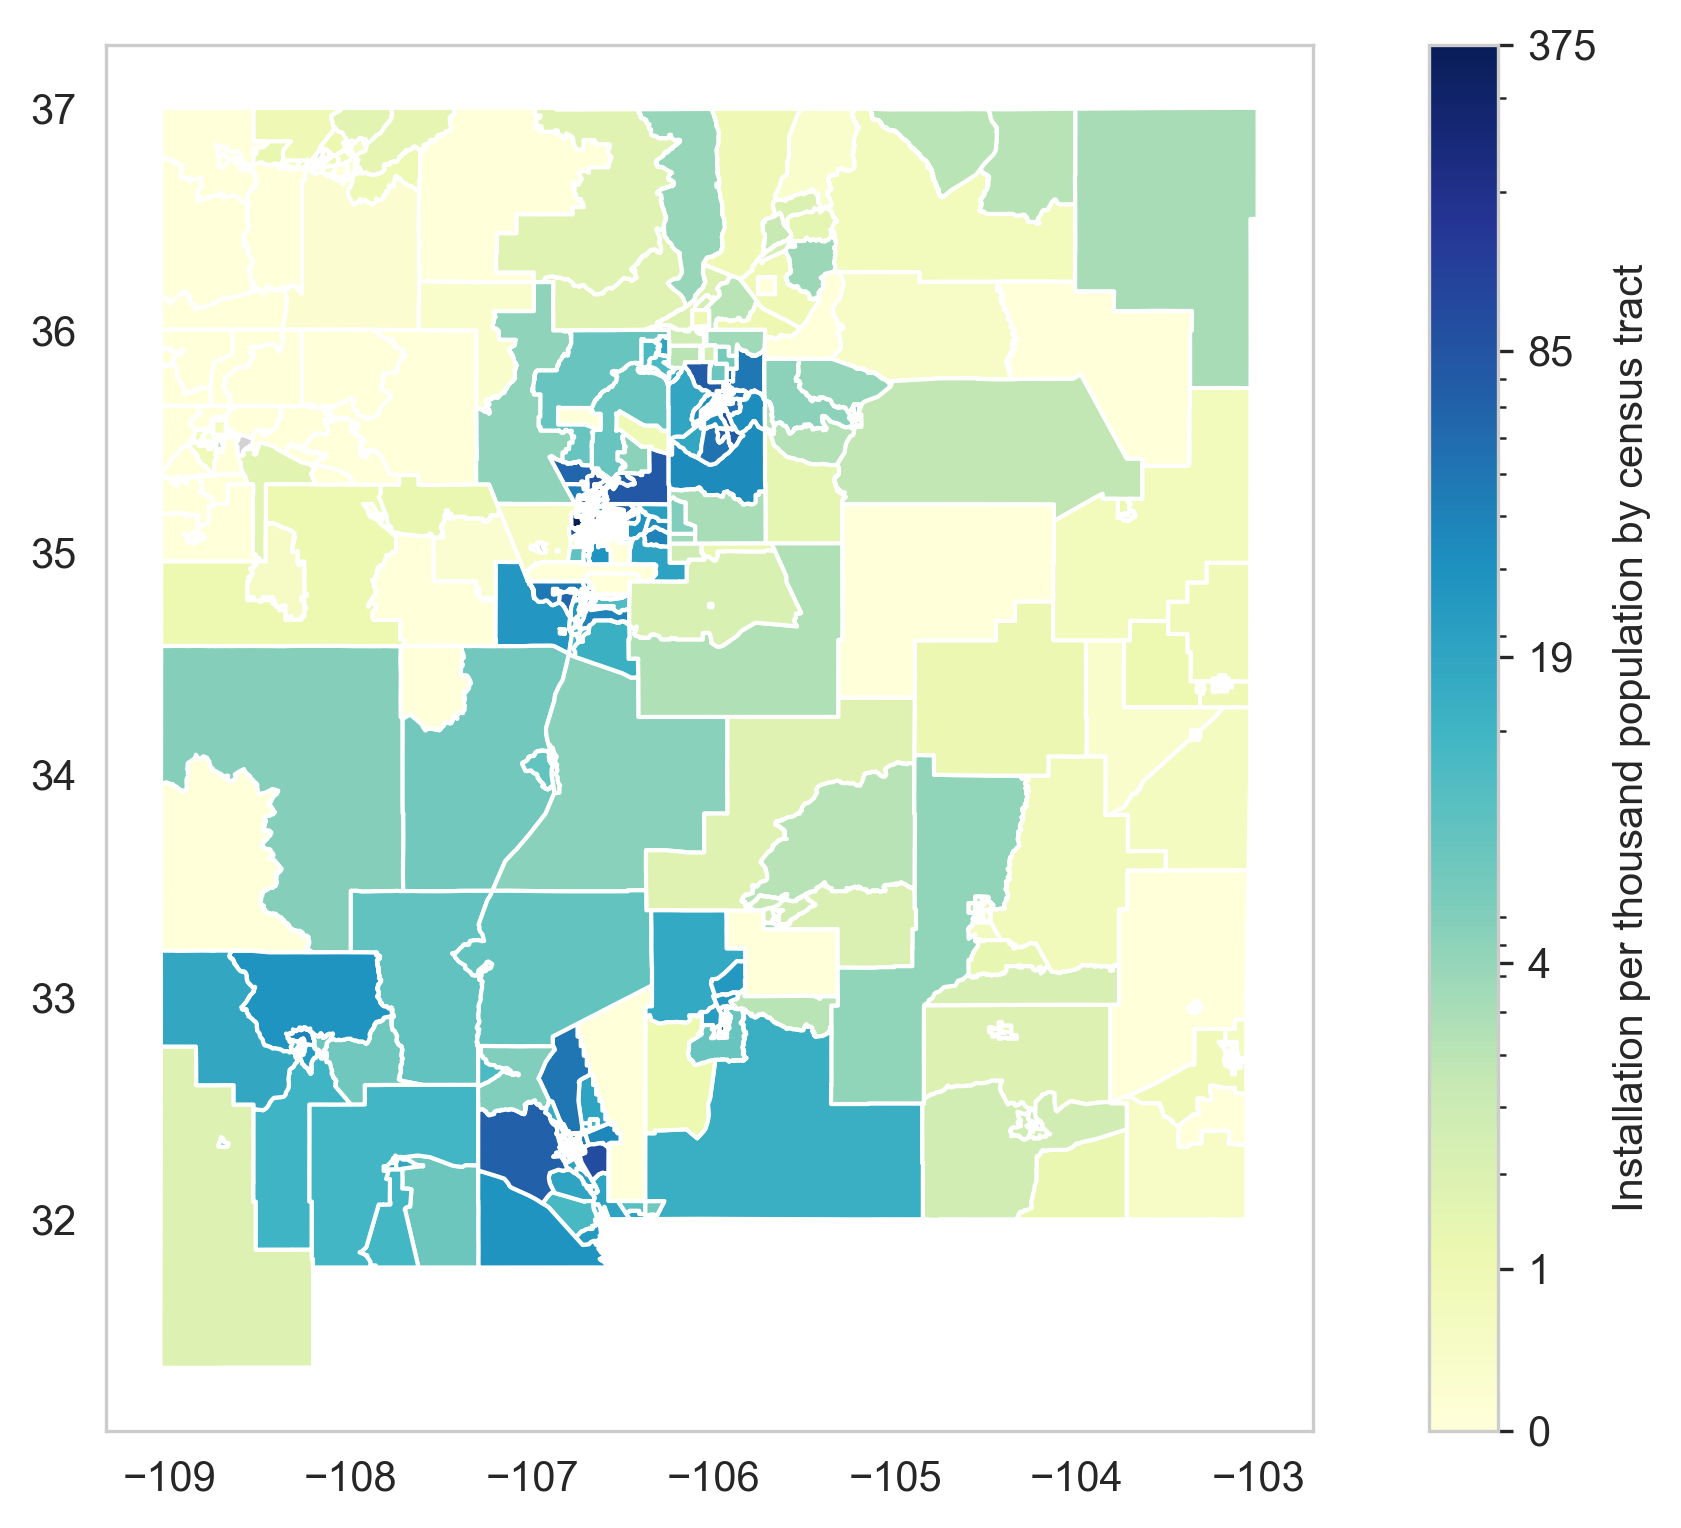
\includegraphics[width=1\textwidth]{figures/tract_count_per_kpop_map.png}
    \caption{Installation per thousand population by 2020 census tract}
    \label{fig:install_kpop}
      \begin{flushleft}
        \footnotesize Note: Population is taken at the 2022 level.
    \end{flushleft}
\end{figure}

\begin{figure}[H]
    \centering
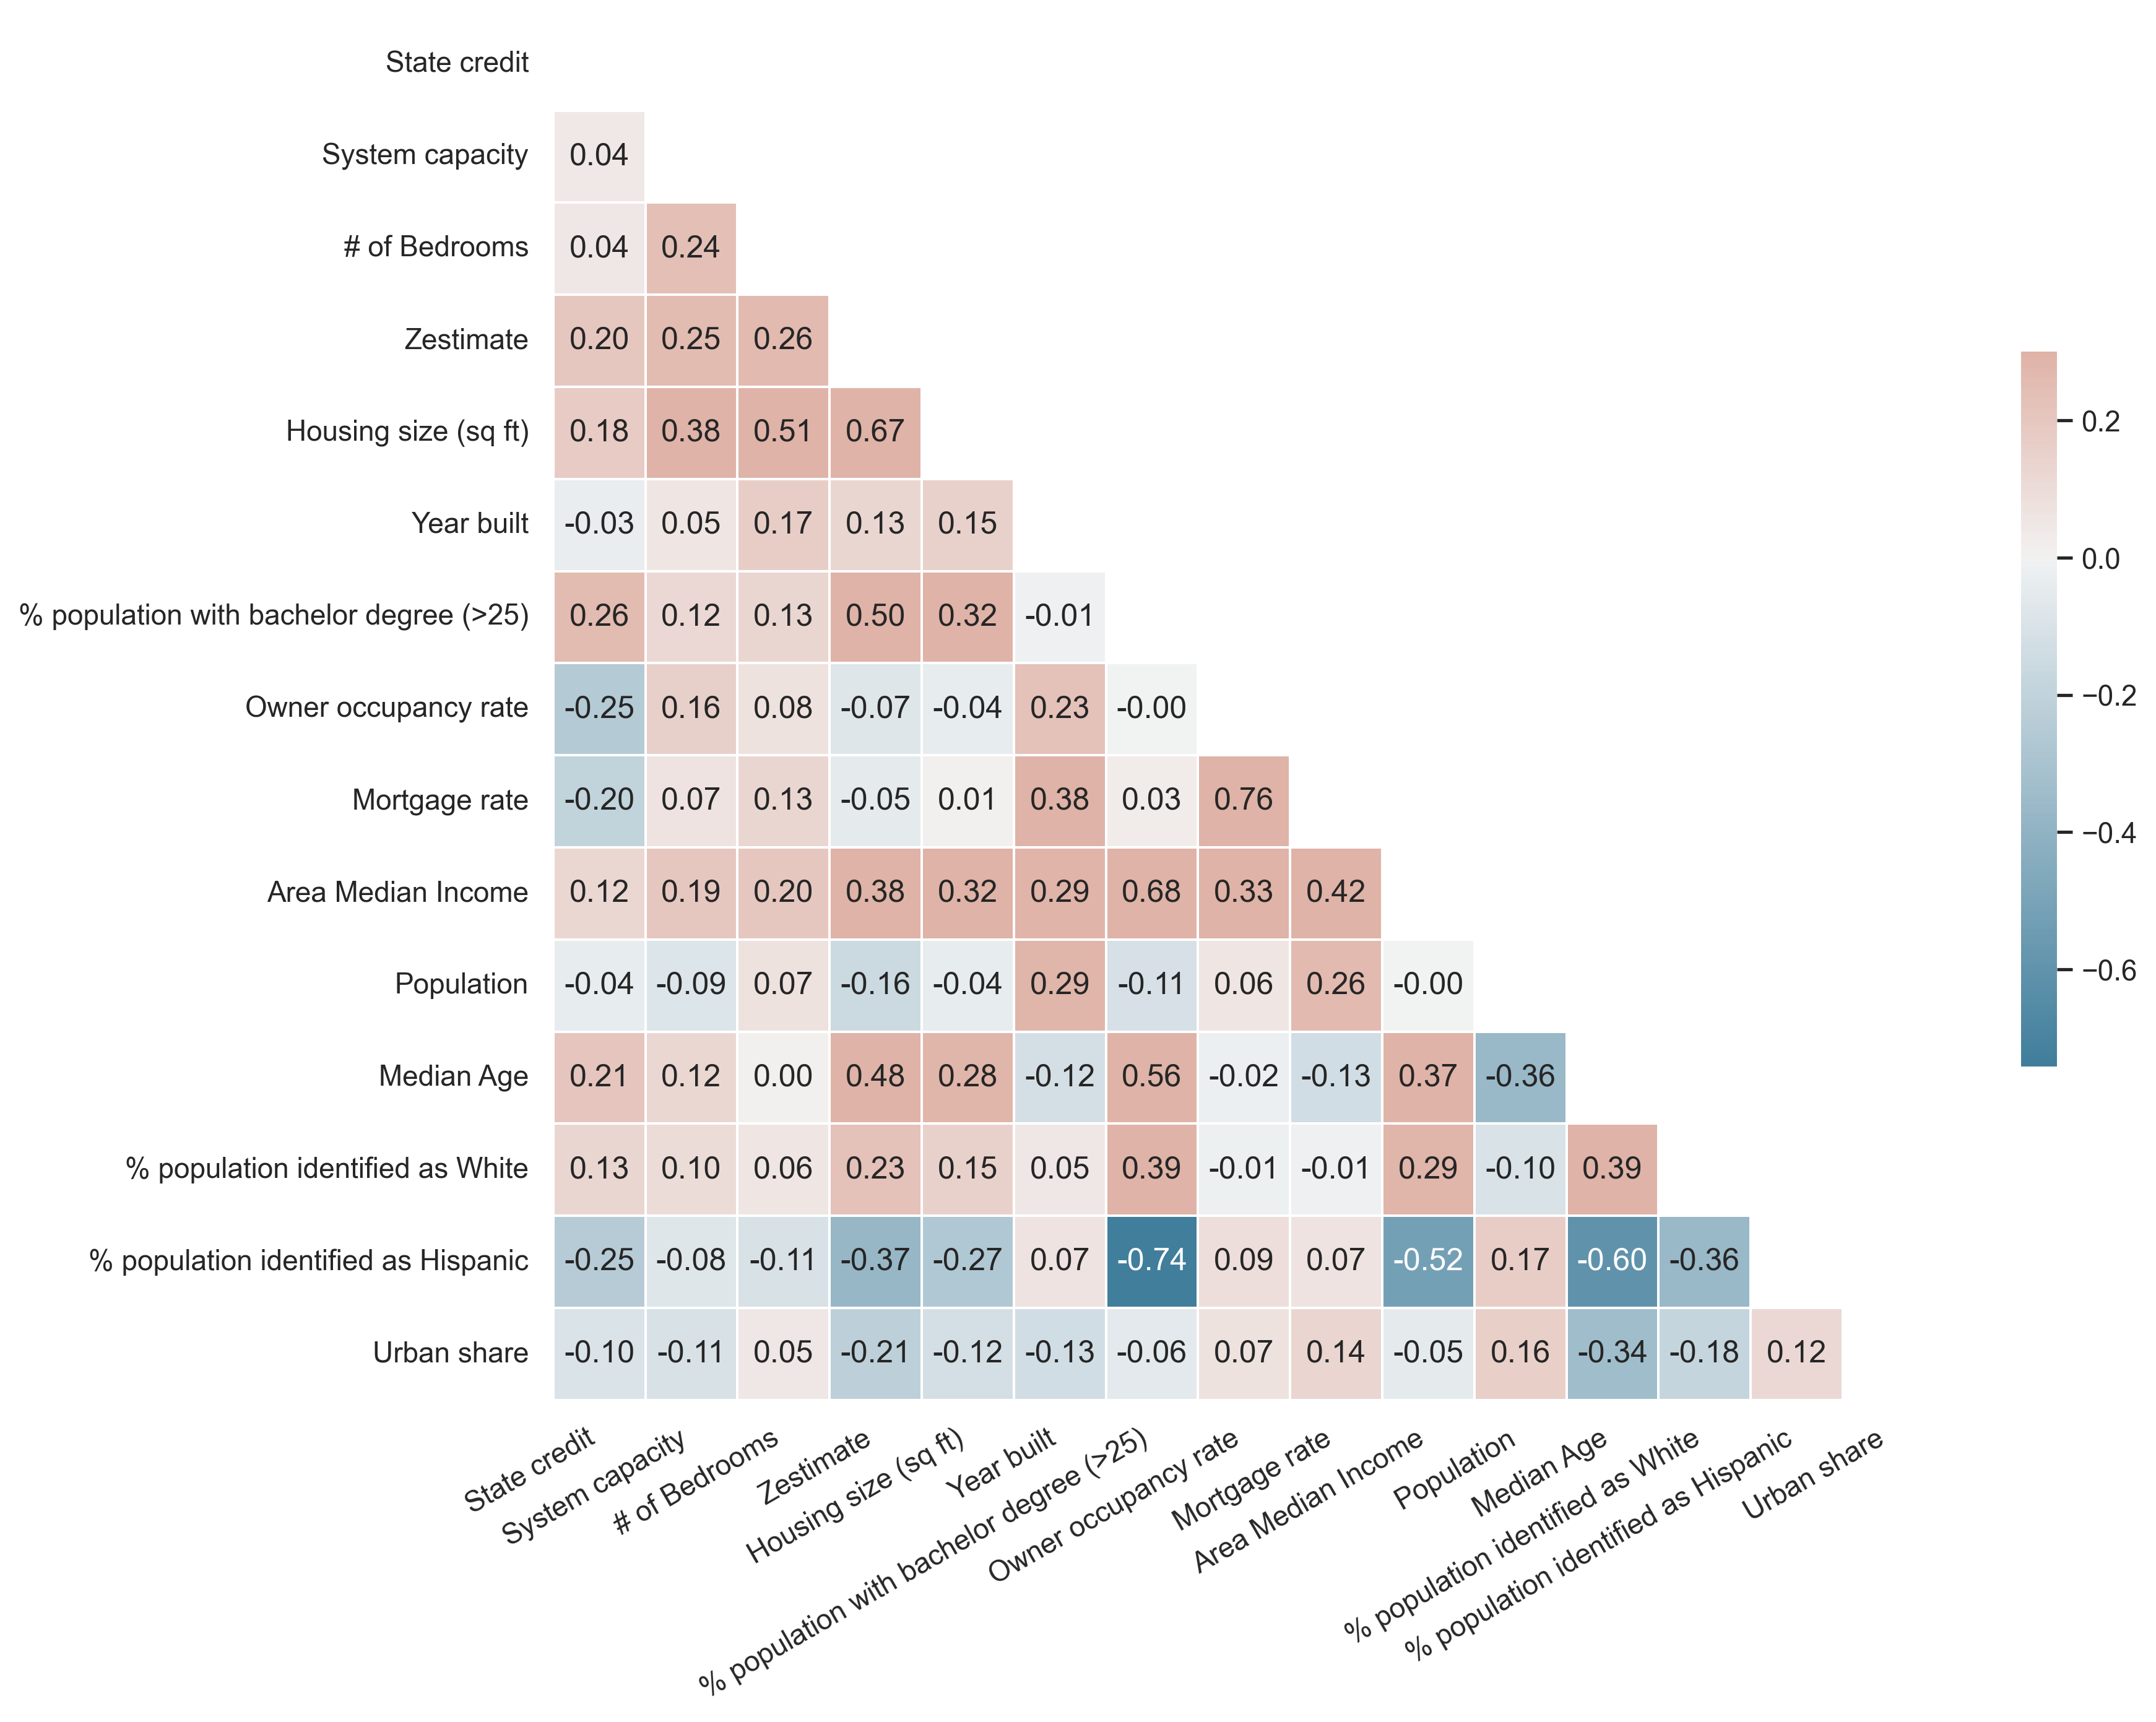
\includegraphics[width=1\textwidth]{figures/corr_matrix.png}
    \caption{Correlation matrix between regression variables}
    \label{fig:corr_matrix}
\end{figure}

\begin{figure}[!ht]
    \centering
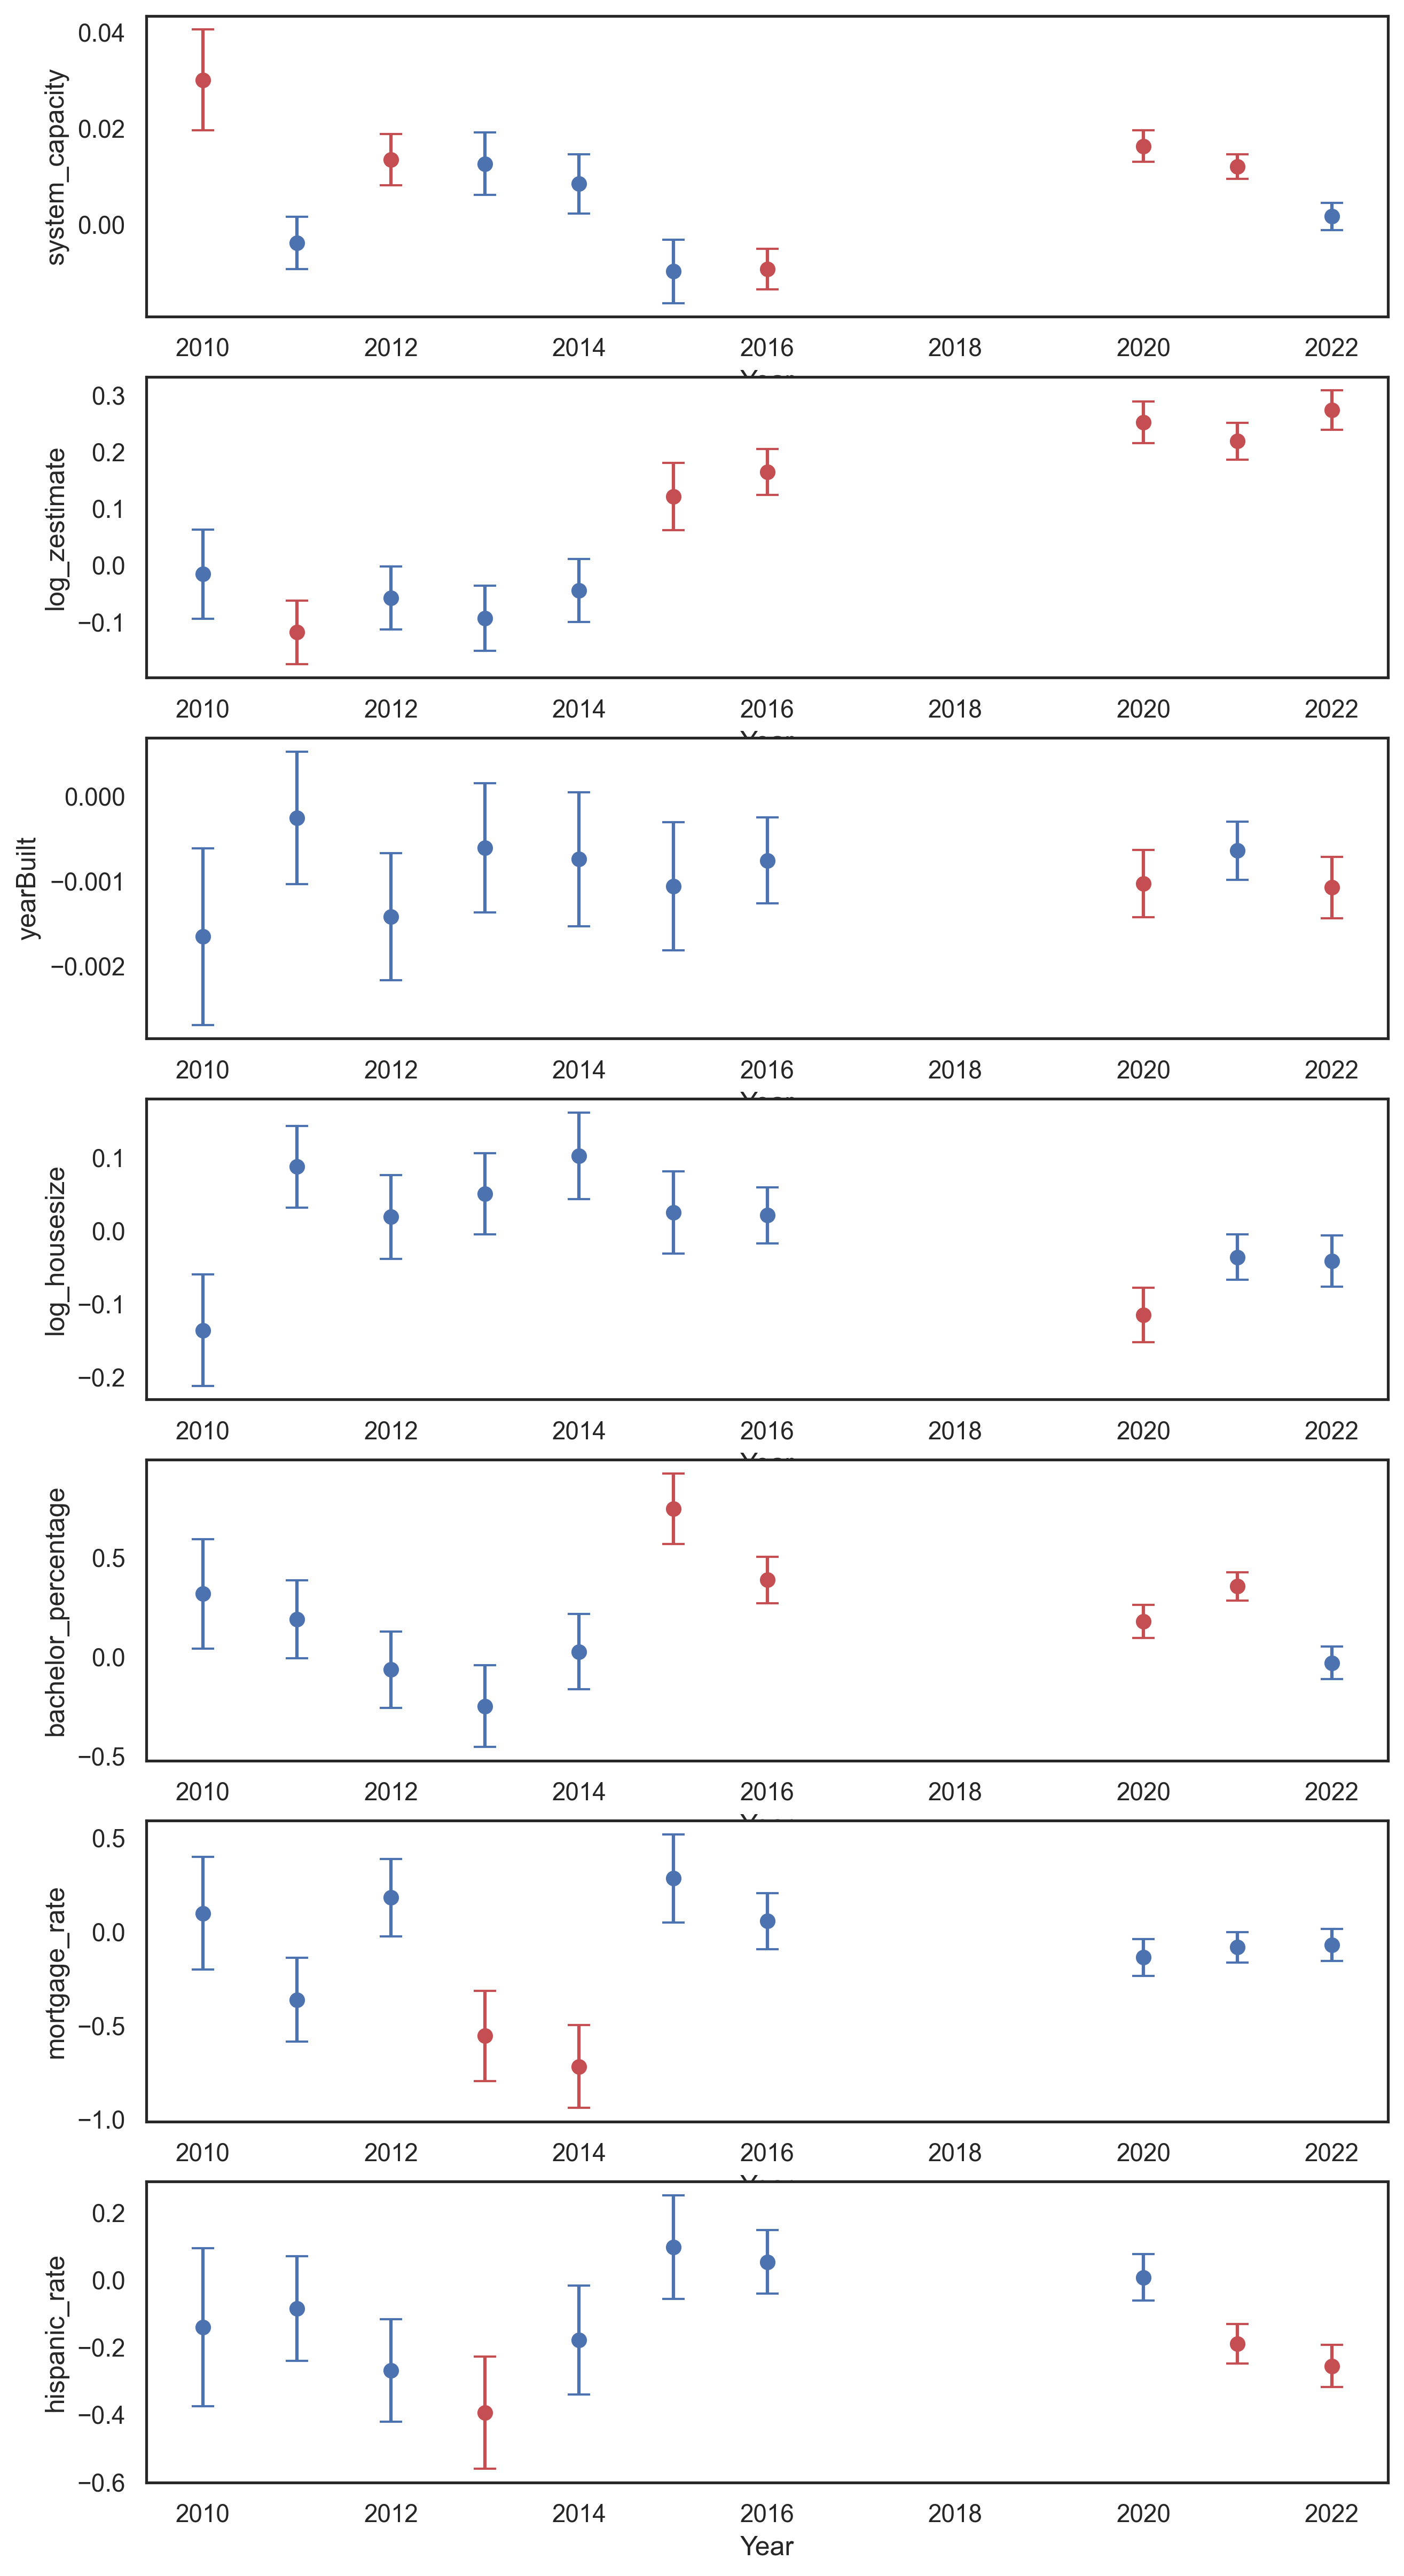
\includegraphics[width=0.7\textwidth]{figures/coefficient_trend.png}
    \caption{Coefficient trend by year}
    \label{fig:coefficient_trend}
\end{figure}




%%%%%%%%%%%%%%%%%%%%%%%%%%%%%%%%%%%
\newpage

\printbibliography

\end{document}
